\documentclass[10pt,conference,compsocconf]{IEEEtran}

\usepackage[
backend=biber,
%style=alphabetic,
%sorting=ynt
]{biblatex}

\usepackage{float}
\usepackage{url}
\usepackage{graphicx}	% For figure environment
\usepackage{booktabs}
\usepackage{amsmath}

\usepackage{subcaption}
\usepackage{hyperref}
\usepackage{pdfpages}
\usepackage{enumerate}
\usepackage{subcaption}
\usepackage{cleveref}

\clubpenalty=-100
%\windowpenalty=-100
\displaywidowpenalty=-100 
\linepenalty=5000
\clubpenalty=10000
\widowpenalty=10000
\displaywidowpenalty=10000


\renewcommand\thesection{Q\arabic{section}}

\addbibresource{ML4Healthcare.bib}
\defbibheading{references}{\section*{\large References}}

\title{Heart Disease Prediction and Pneumonia Prediction \\
\large Interpretable and Explainable Classification for Medical Data \\
\normalsize Project 1 for the Machine Learning for Health Care course (261-5120-00L) \\ \vspace*{20pt}
April 2023
}

\author{
  Sofie Daniëls, Juraj Micko\\
  Group: 3 \\
  Department of Computer Science, ETH Zurich, Switzerland
}

\begin{document}
\pagenumbering{arabic}
\maketitle
\thispagestyle{plain}
\pagestyle{plain}



%\begin{abstract}
%  abc
%\end{abstract}

\section*{\large PART 1: HEART DISEASE PREDICTION}
\section{Exploratory Data Analysis}

In this project, we work with the Heart Failure Prediction Dataset \cite{HeartFailurePrediction} on Kaggle, according to which ``Heart failure is a common event caused by CVDs and this dataset contains 11 features that can be used to predict a possible heart disease.''

The dataset contains $184$ rows of data. By inspection of the dataset columns, we split the features into numerical and categorical. The \textbf{numerical} features are:
\begin{itemize}
    \item \texttt{Age} -- all are integer values between 28 and 75, with no missing values, and a distribution close to normal.
    \item \texttt{RestingBP} -- integer values between 92--200, resembling a normal distribution. No missing values.
    \item \texttt{Cholesterol} -- integer values between 100--603, however, the column contains 31 missing values.
    \item \texttt{MaxHR} -- integer value between 71--202, close to normally distributed; no missing values.
    \item \texttt{Oldpeak} -- float values between $-2.6$--$4.0$. The distribution has more mass at the value $0.0$ suggesting that maybe some NaN values were formatted as $0.0$, but since there is no way for us to distinguish a NaN value from $0.0$, we decided to not process this further.
\end{itemize}
\begin{figure}[H]
    \centering
    \begin{subfigure}{0.19\columnwidth}
        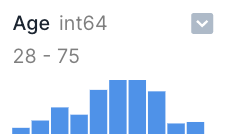
\includegraphics[width=1\textwidth]{images/feat_age.png}
    \end{subfigure}
    \begin{subfigure}{0.19\columnwidth}
        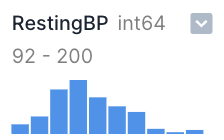
\includegraphics[width=1\textwidth]{images/feat_restingbp.png}
    \end{subfigure}
    \begin{subfigure}{0.19\columnwidth}
        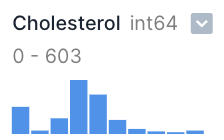
\includegraphics[width=1\textwidth]{images/feat_cholesterol.png}
    \end{subfigure}
    \begin{subfigure}{0.19\columnwidth}
        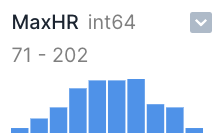
\includegraphics[width=1\textwidth]{images/feat_maxhr.png}
    \end{subfigure}
    \begin{subfigure}{0.19\columnwidth}
        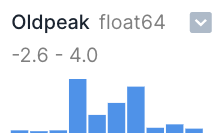
\includegraphics[width=1\textwidth]{images/feat_oldpeak.png}
    \end{subfigure}
    \caption{Visualized distributions of the numerical features.}
\end{figure}

The categorical features include:
\begin{enumerate}
    \item \texttt{Sex} -- admits values \texttt{M} ($82.6\%$, \texttt{F} with no missing values.
    \item \texttt{ChestPainType} -- admits values \texttt{ASY} (most common with $115$ instances), \texttt{NAP}, \texttt{ATA}, \texttt{TA}; no missing values.
    \item \texttt{FastingBS} -- admits values \texttt{0}, \texttt{1}. This feature is formatted as integers, so there is no need to transform it into a numerical value.
    \item \texttt{RestingECG} -- admits values \texttt{Normal} (most common), \texttt{LVH}, \texttt{ST}.
    \texttt{ExerciseAngina} -- a boolean feature with values \texttt{Y}, \texttt{N}.
    \item \texttt{ST\_Slope} -- has values \texttt{Flat} (most common), \texttt{Up}, \texttt{Down}.
\end{enumerate}
No categorical features have missing values.

Finally, the dataset has the column \texttt{HeartDisease} with values either \texttt{0} ($59.8\%$) and \texttt{1} ($40.2\%$), which is our target feature to predict. We observe that the classes are imbalanced. We account for that in the models described in the later sections by using the F1 score for evaluation.

\subsection{Data preprocessing}

For numerical features, we impute in missing values in the dataset using k-Nearest Neighbors (with $k=2$ and uniform weights).

Categorical features are encoded using one-hot encoding with one output feature for each class in the input. An exception are binary categorical features (namely \texttt{Sex} and \texttt{ExerciseAngina}) that are mapped only to a single binary numerical feature. Further, we decided to map values of the \texttt{ST\_Slope} feature by
\begin{align*}
\texttt{Up}\ &\mapsto\ 1\\
\texttt{Flat}\ &\mapsto\ 0\\
\texttt{Down}\ &\mapsto\ -1
\end{align*}
to allow models to make use of the ordinal relationship between the labels of this feature.
Using the described expands the 11 input features (mixed numerical and categorical) into 16 numerical features, see \autoref{fig:preprocessing_pipeline}.

\begin{figure}
    \centering
    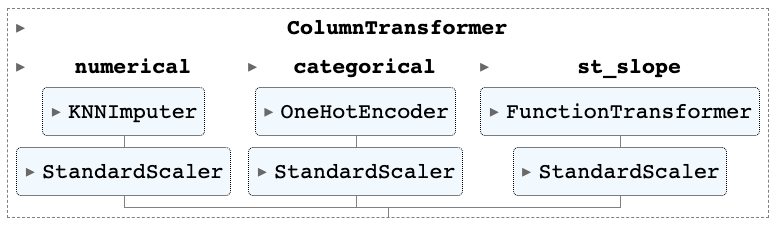
\includegraphics[width=1\columnwidth]{images/preprocessor_pipeline.png}
    \caption{Diagram showing the preprocessing pipeline}
    \label{fig:preprocessing_pipeline}
\end{figure}

Finally, we standardize the feature values by removing their mean and scaling them to unit variance.

\subsection{Train-Test Split}

We split the $184$ samples in the input dataset by $75\%/25\%$ randomly into a train dataset ($138$ samples) and a test dataset ($46$ samples). The operation, as well as all other random operations in the project, is deterministic and thus reproducible using a constant seed.

\subsection{First insights}

Figures \ref{fig:numerical_correlations} and \ref{fig:all_correlations} show correlation matrices between all features (including the target feature \texttt{HeartDisease}). From those, we observe that the most relevant features for heart disease prediction are: \texttt{ST\_Slope}, \texttt{ExerciseAngina}, \texttt{ChestPainType}, \texttt{MaxHR}. This suggests that models relying on these features for prediction will achieve a higher score.

\begin{figure}
    \centering
    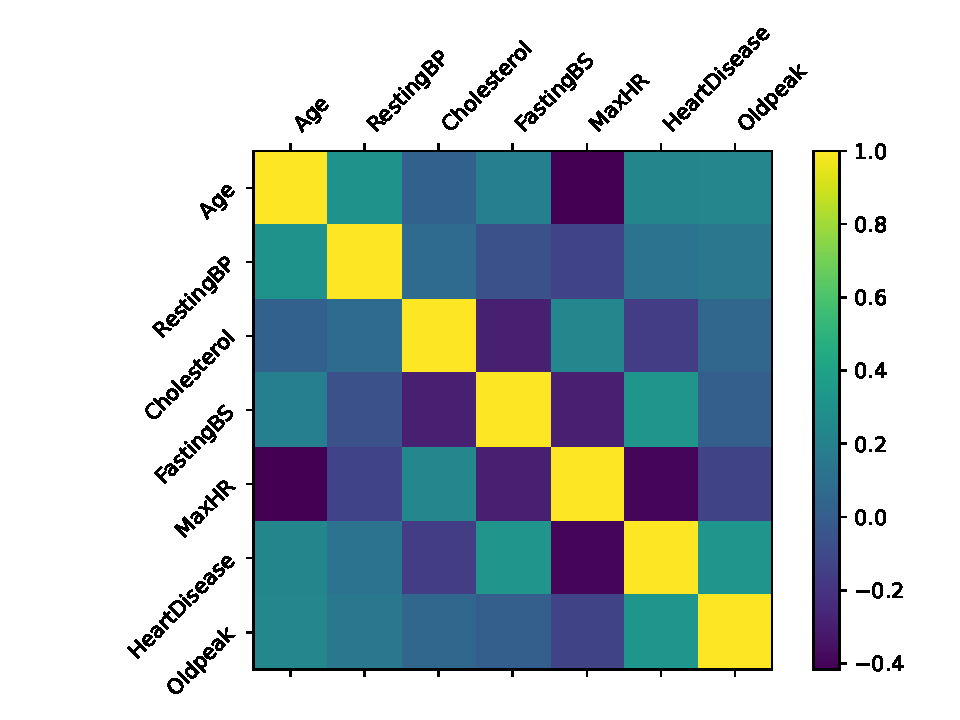
\includegraphics[width=1\columnwidth]{images/numerical_correlations.pdf}
    \caption{Correlation matrix of the numerical features}
    \label{fig:numerical_correlations}
\end{figure}
\begin{figure}
    \centering
    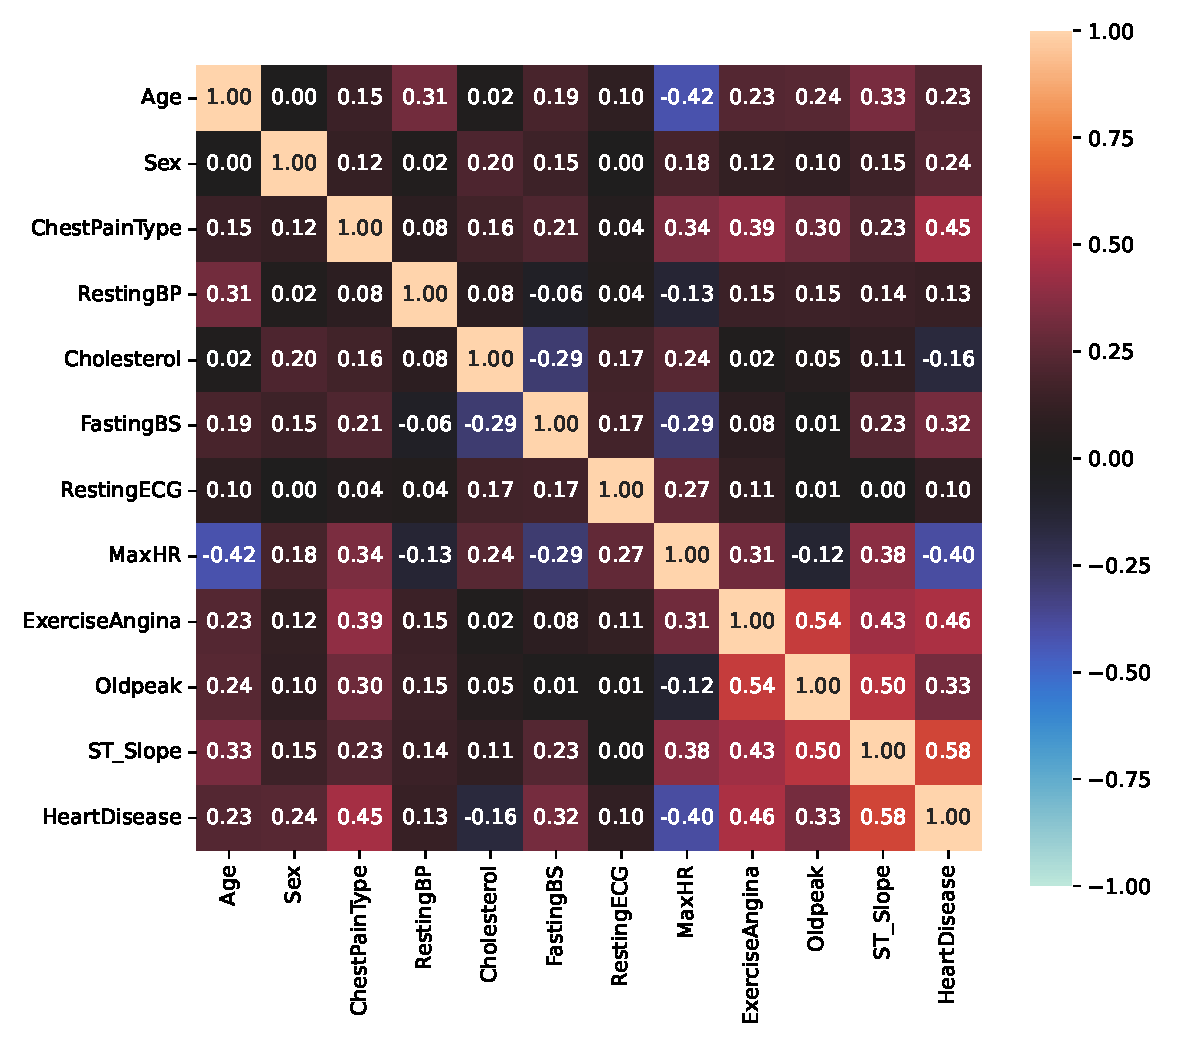
\includegraphics[width=1\columnwidth]{images/all_correlations.pdf}
    \caption{Convolution matrix of both numerical and categorical features using the \texttt{dython} Python library \cite{zychlinskiDython2023}, which uses ``Pearson's R for numerical-numerical cases, Correlation Ratio for categorical-numerical cases, and Cramer's V for categorical-categorical cases''.}
    \label{fig:all_correlations}
\end{figure}
\begin{figure*}
    \centering
    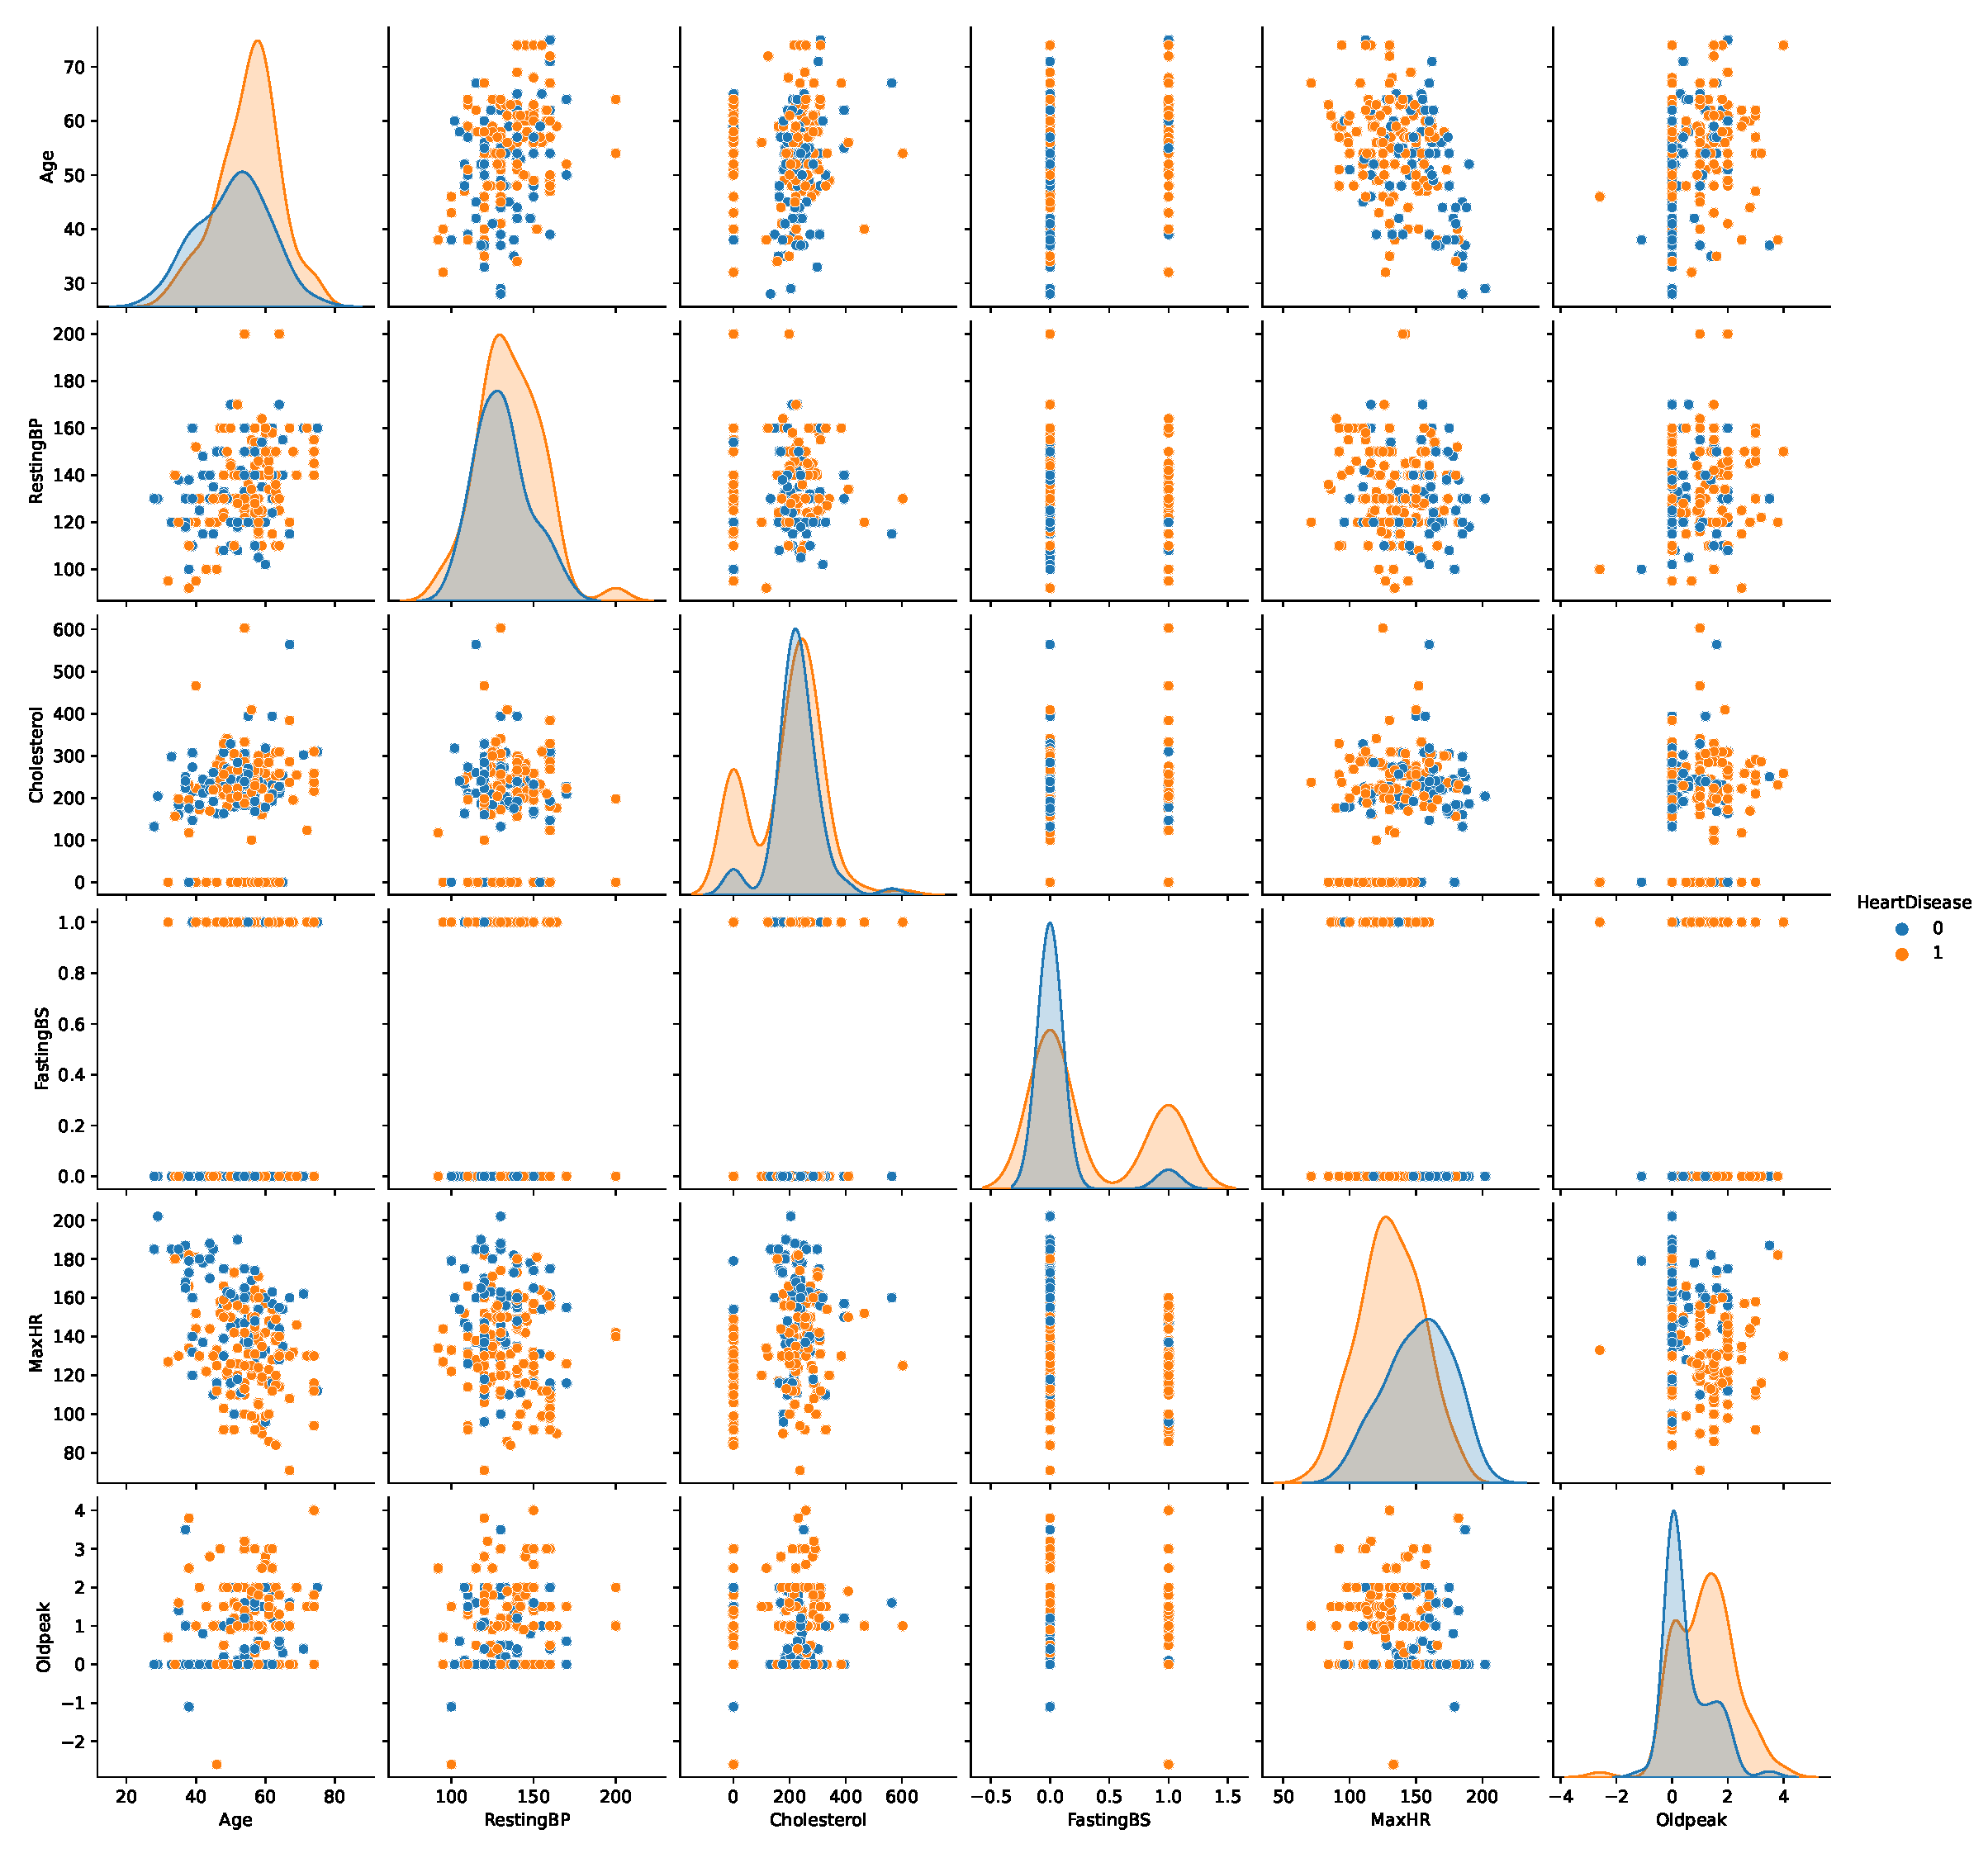
\includegraphics[width=1\textwidth]{images/pairplot.pdf}
    \caption{A plot showing pairwise relationships between numerical features in the dataset. Blue points represent samples without heart disease; orange points represent samples with heart disease.}
    \label{fig:pairplot}
\end{figure*}

\begin{figure}
    \centering
    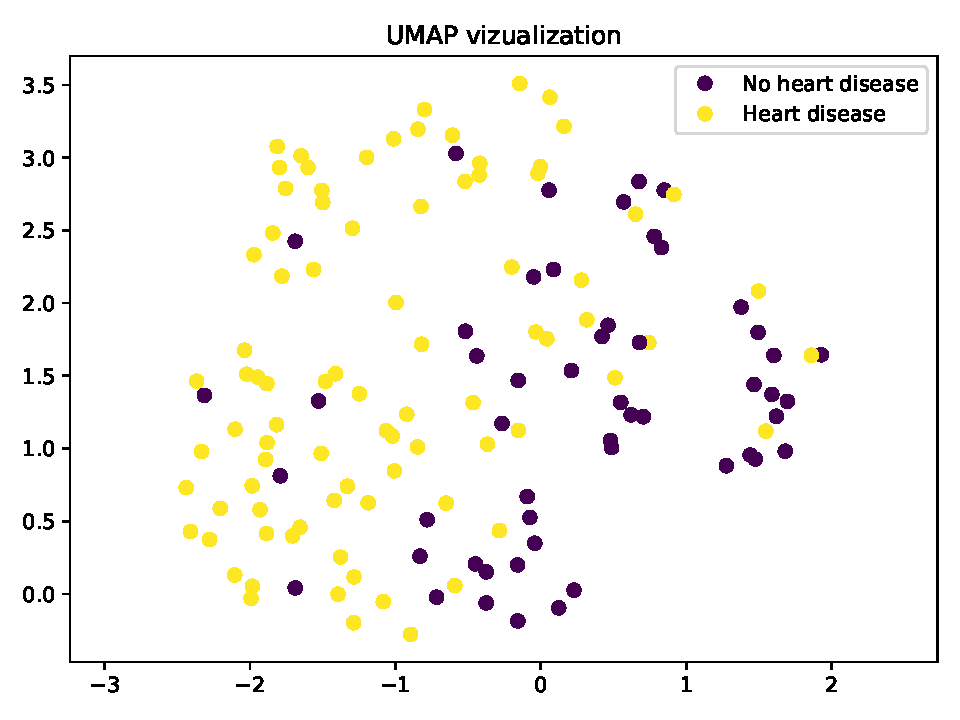
\includegraphics[width=1\columnwidth]{images/umap.pdf}
    \caption{The UMAP visualization \cite{mcinnesUMAPUniformManifold2020} of the training dataset in 2D.}
    \label{fig:umap}
\end{figure}

We also attach pairwise plots in \autoref{fig:pairplot}, which highlights the dependency of some features. As an example, the \texttt{Age}-\texttt{MaxHR} plot explains the negative correlation between the two features.

Additionally, in \autoref{fig:umap}, we analyze the training dataset visually using the UMAP dimensionality reduction tool \cite{mcinnesUMAPUniformManifold2020}. We observe that the dataset is at least to some extent linearly separable after the UMAP transformation even in two dimensions, which gives us an estimate of how well a good model should perform.

\section{Logistic Lasso Regression}
\label{sec:p1q2}

An important preprocessing step for Lasso regression (i.e. Logistic regression with the $L_1$-regularization) is the standardization of the features, which has been done in the preprocessing step.

We trained a Lasso regression classifier using a logistic model with SGD training and $L_1$-regularization. The loss function is set to log-loss which is suitable for binary classification.

We optimized for the $\alpha$ parameter (the amount of $L_1$ regularization) using a grid search on 31 logarithmically-spaced values between $0.001$ and $1$, choosing $\alpha\approx 0.025$. The grid search optimized for the F1 score, by cross-validation within the training dataset.

The model achieved the (F1) score of $85.9\%$ on the training dataset and the score of $79.2\%$ on the test dataset.

\begin{figure*}
    \centering
    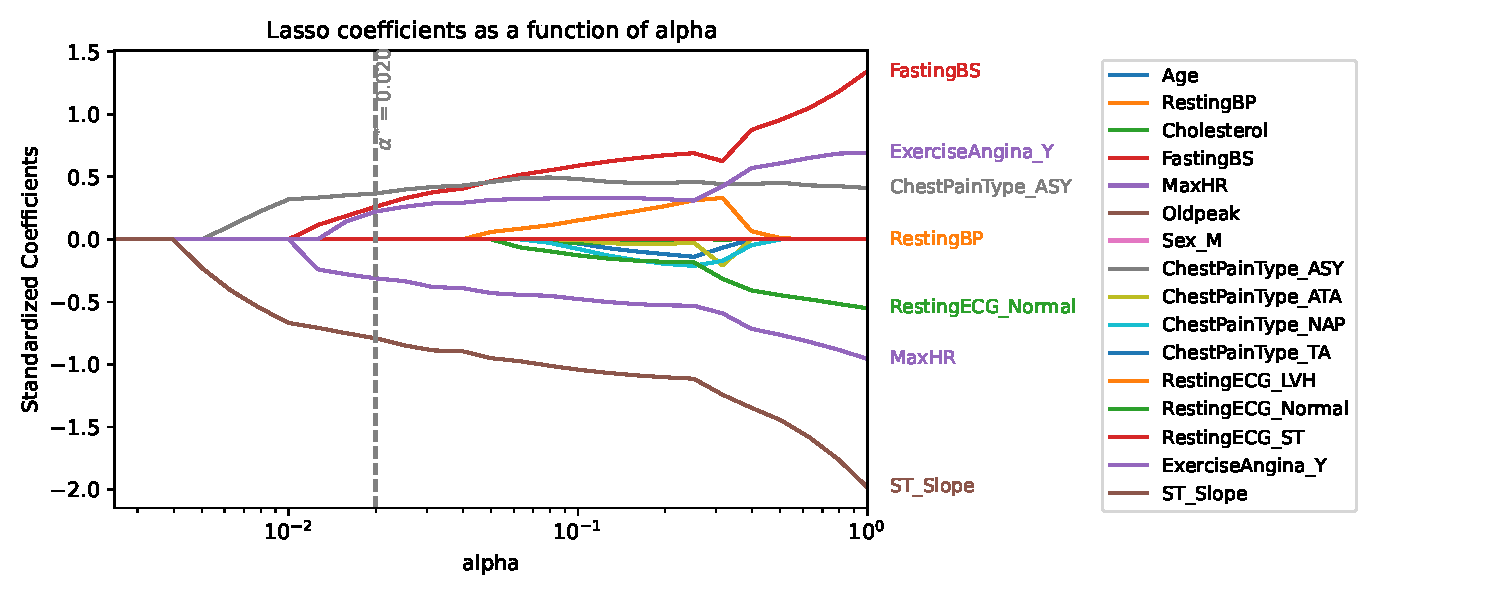
\includegraphics[width=0.9\textwidth]{images/lasso_coef_f.pdf}
    \caption{Lasso coefficients as a function of $\alpha$. The horizontal line corresponds to the highest-scoring $\alpha=0.025$}
    \label{fig:lasso_coef_f}
\end{figure*}

\autoref{fig:lasso_coef_f} shows the importance of each feature for each considered value of $\alpha$. We observe that with decreasing $\alpha$, the model has more features with positive coefficients, as expected.

We also observe that the set of features highly correlated with Heart disease is similar to those marked as most relevant by the Lasso regression, i.e. those with positive coefficients at $\alpha=0.025$. Namely, the features marked as relevant by Lasso regression are: \texttt{ST\_Slope}, \texttt{ChestPainType\_ASY} (a one-hot flag of the \texttt{ChestPainType} feature), \texttt{MaxHR}, \texttt{FastingBS}, and \texttt{ExerciseAngina\_Y}.

Further, we attempted fitting another Lasso regression which would only use those features marked as relevant. For this second regression, a similar grid-search approach found the same $\alpha$ optimal. The second model achieved slightly higher score on the train dataset, but made no difference on the test dataset; see \autoref{tab:lasso_selection}.

\begin{table}
\centering
\begin{tabular}{l|l|l|}
 & Train (F1) & Test (F1) \\ \hline
Lasso-all & $85.9\%$ & $79.2\%$ \\ \hline
Lasso-selected & $86.0\%$ & \textbf{$79.2\%$} \\ \hline
\end{tabular}
\caption{Comparison of the F1 scores of the Lasso regression with all features, and with only the selected 5 features.}
\label{tab:lasso_selection}
\end{table}

\section{Decision Trees}

Next, we trained a single decision tree classifier on the training dataset, see \autoref{fig:decision_tree}. Using a simple search of numerous values we set max-depth to $3$, which worked well. The model achieves the score of $87.7\%$ in training and $78.3\%$ on the test dataset.

\begin{figure*}
    \centering
    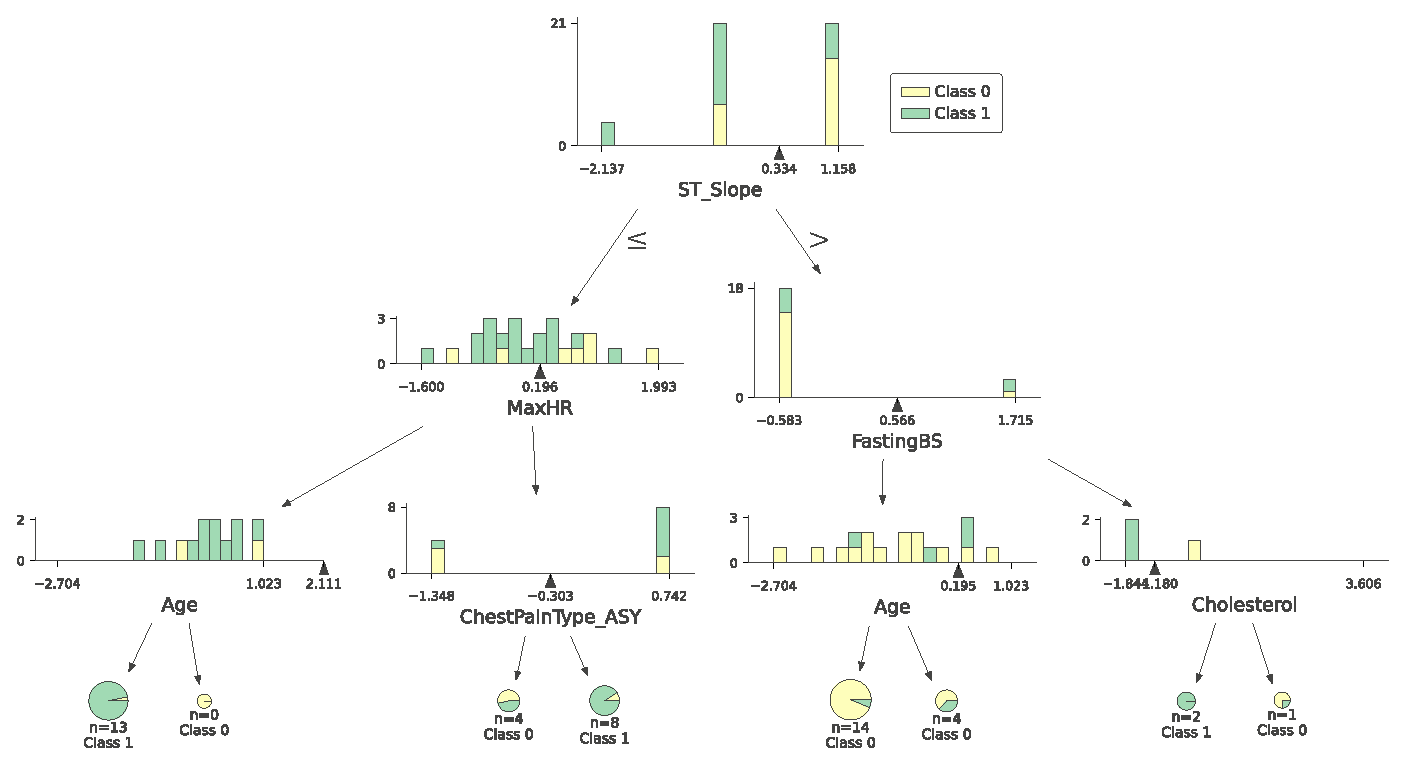
\includegraphics[width=1\textwidth]{images/decision_tree.pdf}
    \caption{A visualization of the trained decision tree.}
    \label{fig:decision_tree}
\end{figure*}

\begin{figure}
    \centering
    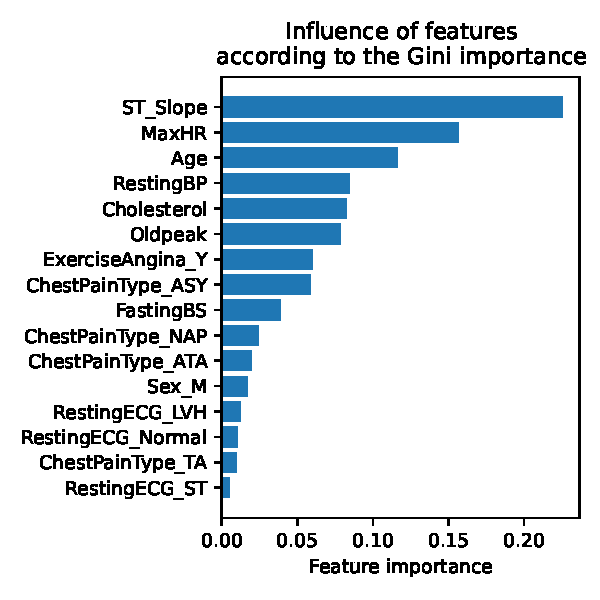
\includegraphics[width=1\columnwidth]{images/random_forest.pdf}
    \caption{A visualization of the influence of the
different features according to the Gini importance.}
    \label{fig:random_forest}
\end{figure}

Further, we trained a random forest classifier using an ensemble of 100 decision trees. In this case, the training data could be learned perfectly, and the achieved test score was $80.4\%$, demonstrating an improvement against a single decision tree.

We visualized the Gini importance of the features in \autoref{fig:random_forest}.


\section{Multi-Layer Perceptrons}

\subsection{Model}

In this part, we implemented a simple multi-layer perceptron network.

We trained the network with the Adam optimizer, and the ReLU activation function was used on all hidden layers.
The batch size was set to $184$, i.e. the whole dataset.

Similar to previous sections, we combined it with grid search and optimized a number of hyper-parameters through cross-validation within the training dataset. We optimized for the following:

\begin{enumerate}[a.]
    \item Architecture. We tried a number of architectures, from smaller single hidden layers (size 8) to multiple bigger layers (size 32). For us the best performing architecture in our setup was a single layer of size 26.
    \item L2 regularization term $\alpha$. We used the L2 regularization (as opposed to L1) because it shrinks feature coefficients evenly and so works better for features that might be codependent. We tried a number of coefficients between $0.1$ and $10$ and achieved the best performance with $\alpha \approx 0.32$.
    \item Learning rate. Out of several values, the best performing was $0.0001$.
    \item The number of epochs was set to 1000, which proved to be enough, while more epochs did not lead to better performance.
\end{enumerate}

\begin{figure}
    \centering
    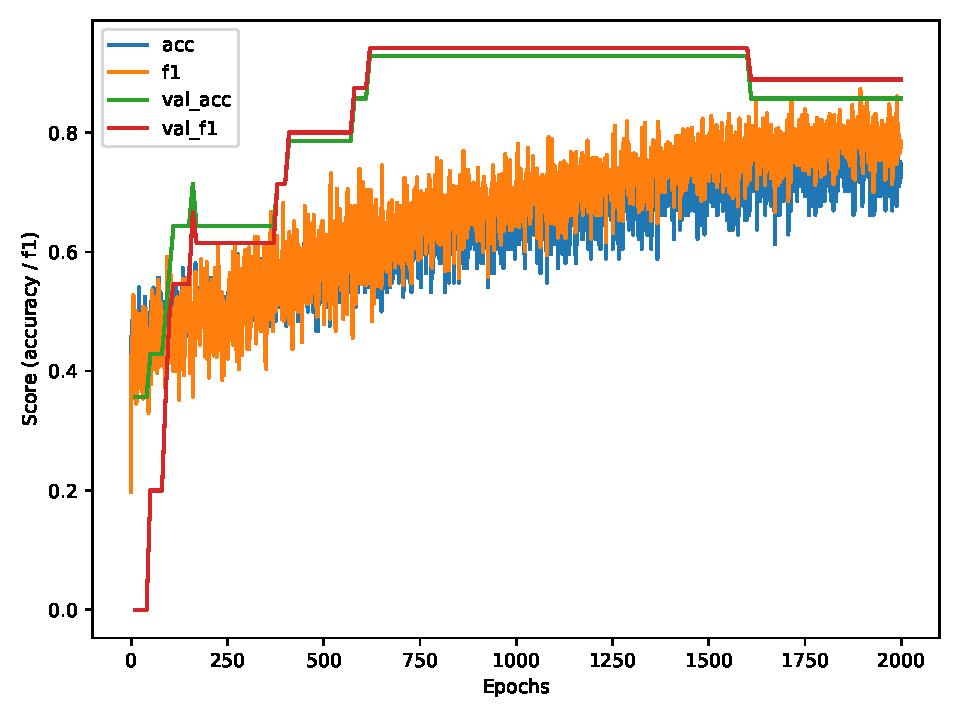
\includegraphics[width=1\columnwidth]{images/mlp_training.pdf}
    \caption{A plot of the training history of the multi-layer perception. On the same axis are the F1 measure and accuracy for comparison. This model was trained only on $90\%$ of the training data to allow the $10\%$ data for validation during training for vizualization purposes. Metrics on the validation data were evaluated every $10$ epochs.}
    \label{fig:mlp_training}
\end{figure}

We also used the dropout value of 0.8, which allowed the model to generalize better, improving the F1 score on the test dataset. \autoref{fig:mlp_training} shows the training history of the MLP. The final model trained on the whole training dataset achieves the F1 score of $0.8$ on the test dataset.

\subsection{Explaining predictions}

In this section, we explain how each feature contributes to predictions of the MLP model. We do so using the SHAP framework \cite{lundbergUnifiedApproachInterpreting2017}.

Of the various explainer algorithms offered by the SHAP Python library, we used the \texttt{Exact} explainer. It is model-agnostic, which fits our use case, and precise since this algorithm does not approximate the result by subsampling. The major disadvantage is the exponential complexity of computing Shapley values in the number of features; however, the computation time is, in practice, feasible for the use case of this project.

We give the explainer as the input the pre-trained MLP model, and the training dataset, which is to be used for masking out feature values during Shapley values calculations. We then feed in the test dataset, on which the Shapley values are calculated.

\begin{figure}
    \centering
    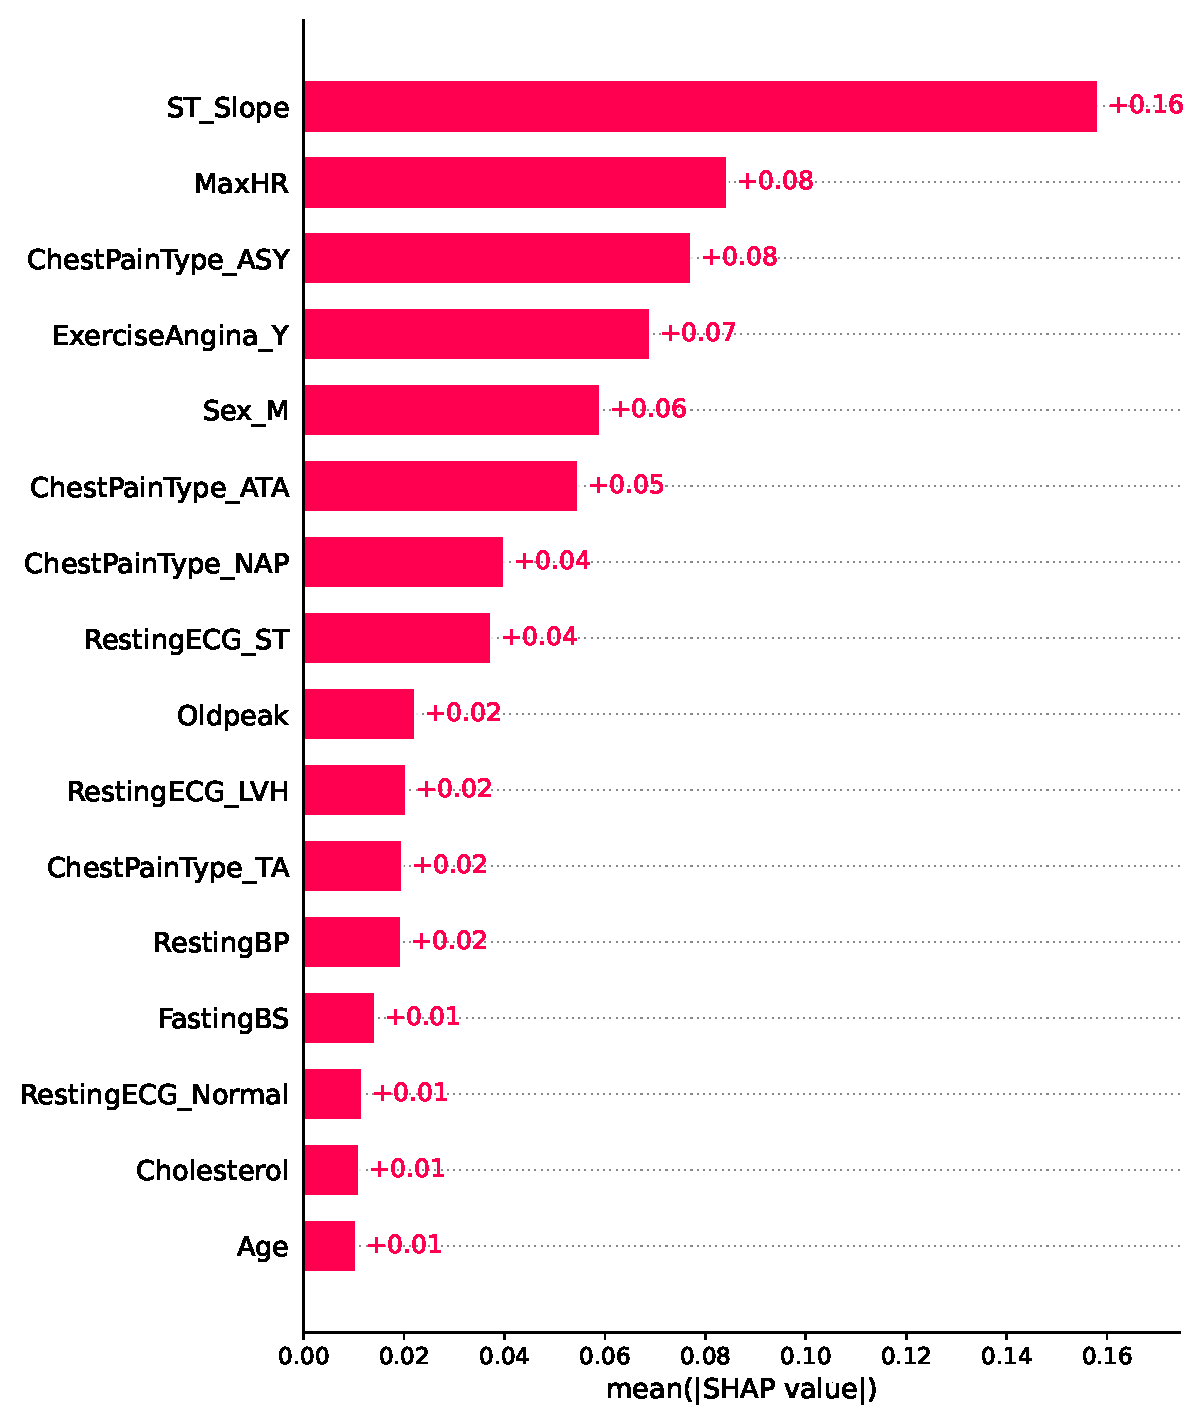
\includegraphics[width=0.8\columnwidth]{images/shap_bar.pdf}
    \caption{Bar vizualization of feature importances of the overall MLP model, averaged on the test dataset.}
    \label{fig:shap_bar}
\end{figure}
\begin{figure}
    \centering
    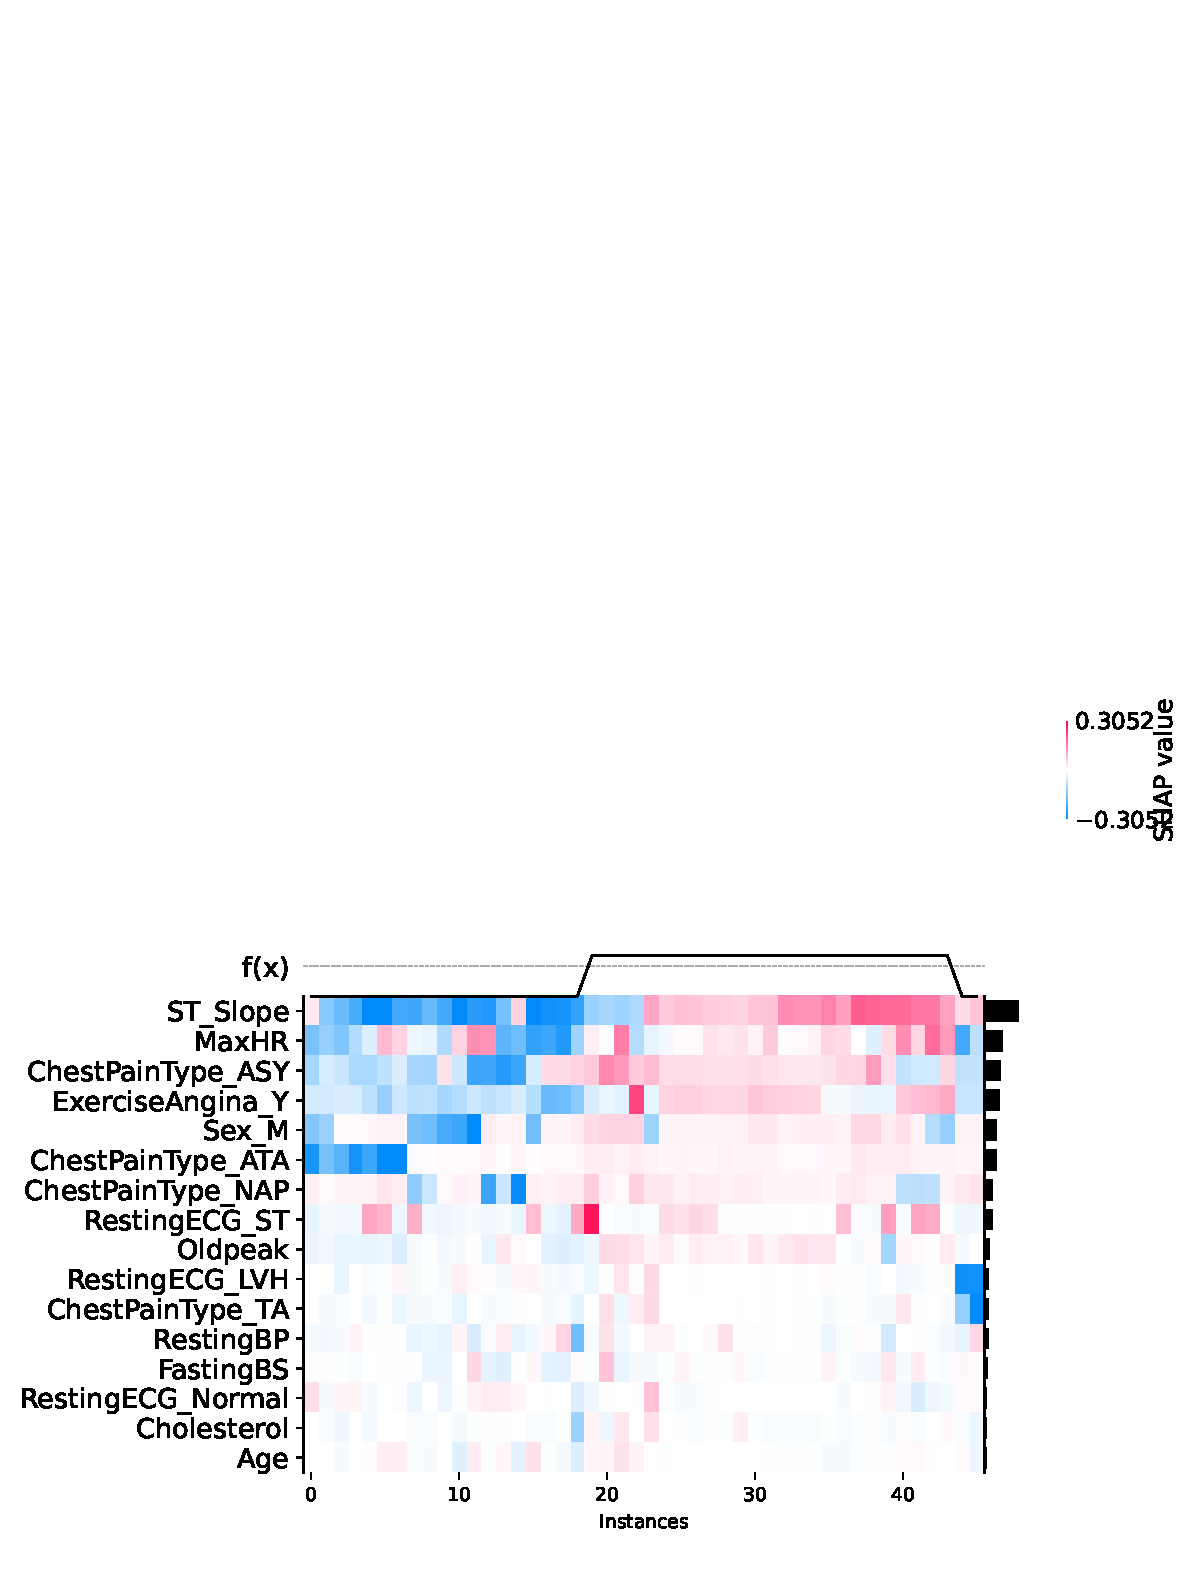
\includegraphics[trim=0 0 2.8cm 16cm,clip,width=1\columnwidth]{images/shap_heatmap.pdf}
    \caption{Heatmap vizualization of per-sample feature importance of the MLP model, on the test dataset. Each cell's color corresponds to the amount the feature (row) influences the prediction of the sample (column). Columns are ordered by hierarchical clustering of the samples. The bars on the right show overall feature importance across the test dataset.}
    \label{fig:shap_heatmap}
\end{figure}
\begin{figure}
    \centering
    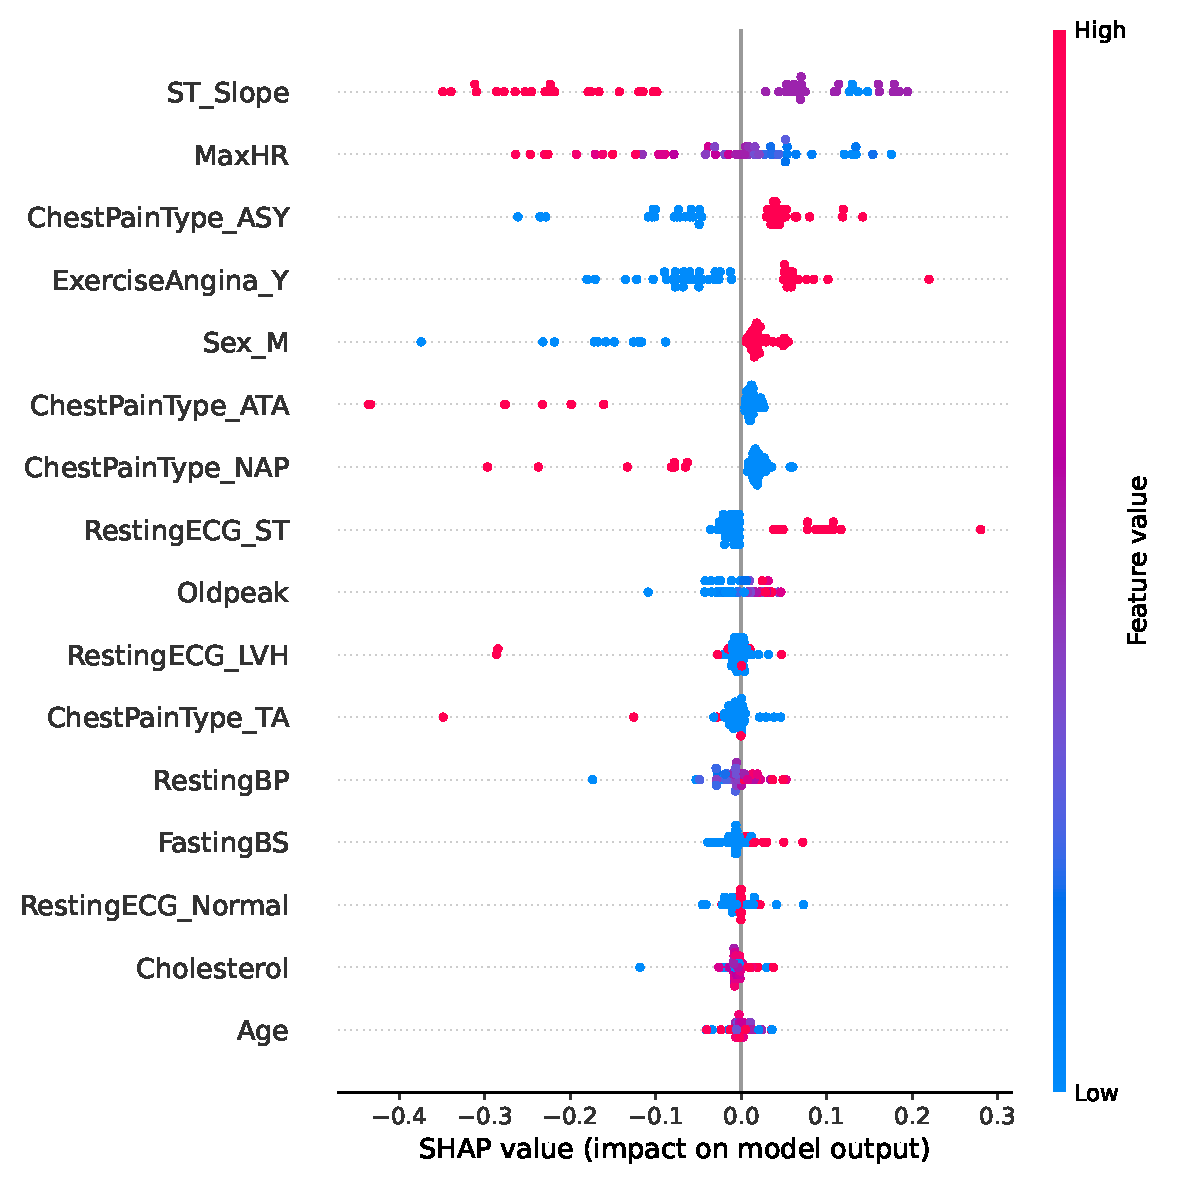
\includegraphics[width=1\columnwidth]{images/shap_beeswarm.pdf}
    \caption{Beeswarm vizualization of feature importances of the overall MLP model on the test dataset. Each marker corresponds to a sample in the test dataset.}
    \label{fig:shap_beeswarm}
\end{figure}
\begin{figure}
    \centering
    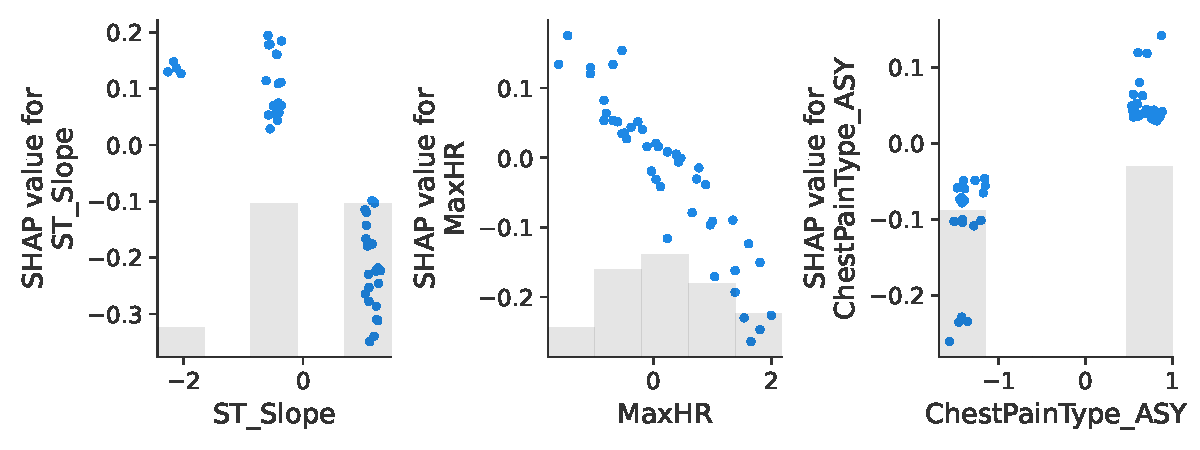
\includegraphics[width=1\columnwidth]{images/shap_scatter.pdf}
    \caption{Scatter plot vizualization of the three most important features according to our SHAP analysis. Individual points correspond to samples in the test dataset. The x-axis is the feature value, and the y-axis is the feature's relative contribution to the final prediction of the sample.}
    \label{fig:shap_scatter}
\end{figure}

\Cref{fig:shap_bar,fig:shap_heatmap,fig:shap_beeswarm} vizualize overall feature importances on the test dataset, using bar (\autoref{fig:shap_bar}), heatmap (\autoref{fig:shap_heatmap}), and beeswarm (\autoref{fig:shap_beeswarm}) plots. \Cref{fig:shap_sample_positive,fig:shap_sample_negative} explain the predictions of four positive and negative samples, respectively.

We note that for the correctly predicted samples, the sets of highly influential features are similar to those identified as important in Q2. Namely, \texttt{ST\_Slope} and \texttt{MaxHR} are each among the top 3 most important features in $5$ out of $6$ correctly predicted samples in \cref{fig:shap_sample_positive,fig:shap_sample_negative}; and \texttt{ChestPainType\_ASY} is among the top $5$ features in $5$ out of $6$ correct predictions. \autoref{fig:shap_scatter} shows a scatter plot of the influence of the three most important features by SHAP.

The features \texttt{Age} and \texttt{RestingBP} which were identified as relatively important according to the Gini importance in Q3, are identified as unimportant according to SHAP (\autoref{fig:shap_bar}).

Further, we observe that feature importances are relatively consistent across different predictions; however, it is usual that a feature generally unimportant according to Q2. becomes responsible for a significant part of the prediction of some feature (e.g. the feature \texttt{Sex\_M} of \autoref{fig:shap_sample_positive_2}).

\begin{figure*}
    \centering
    \begin{subfigure}{1\columnwidth}
        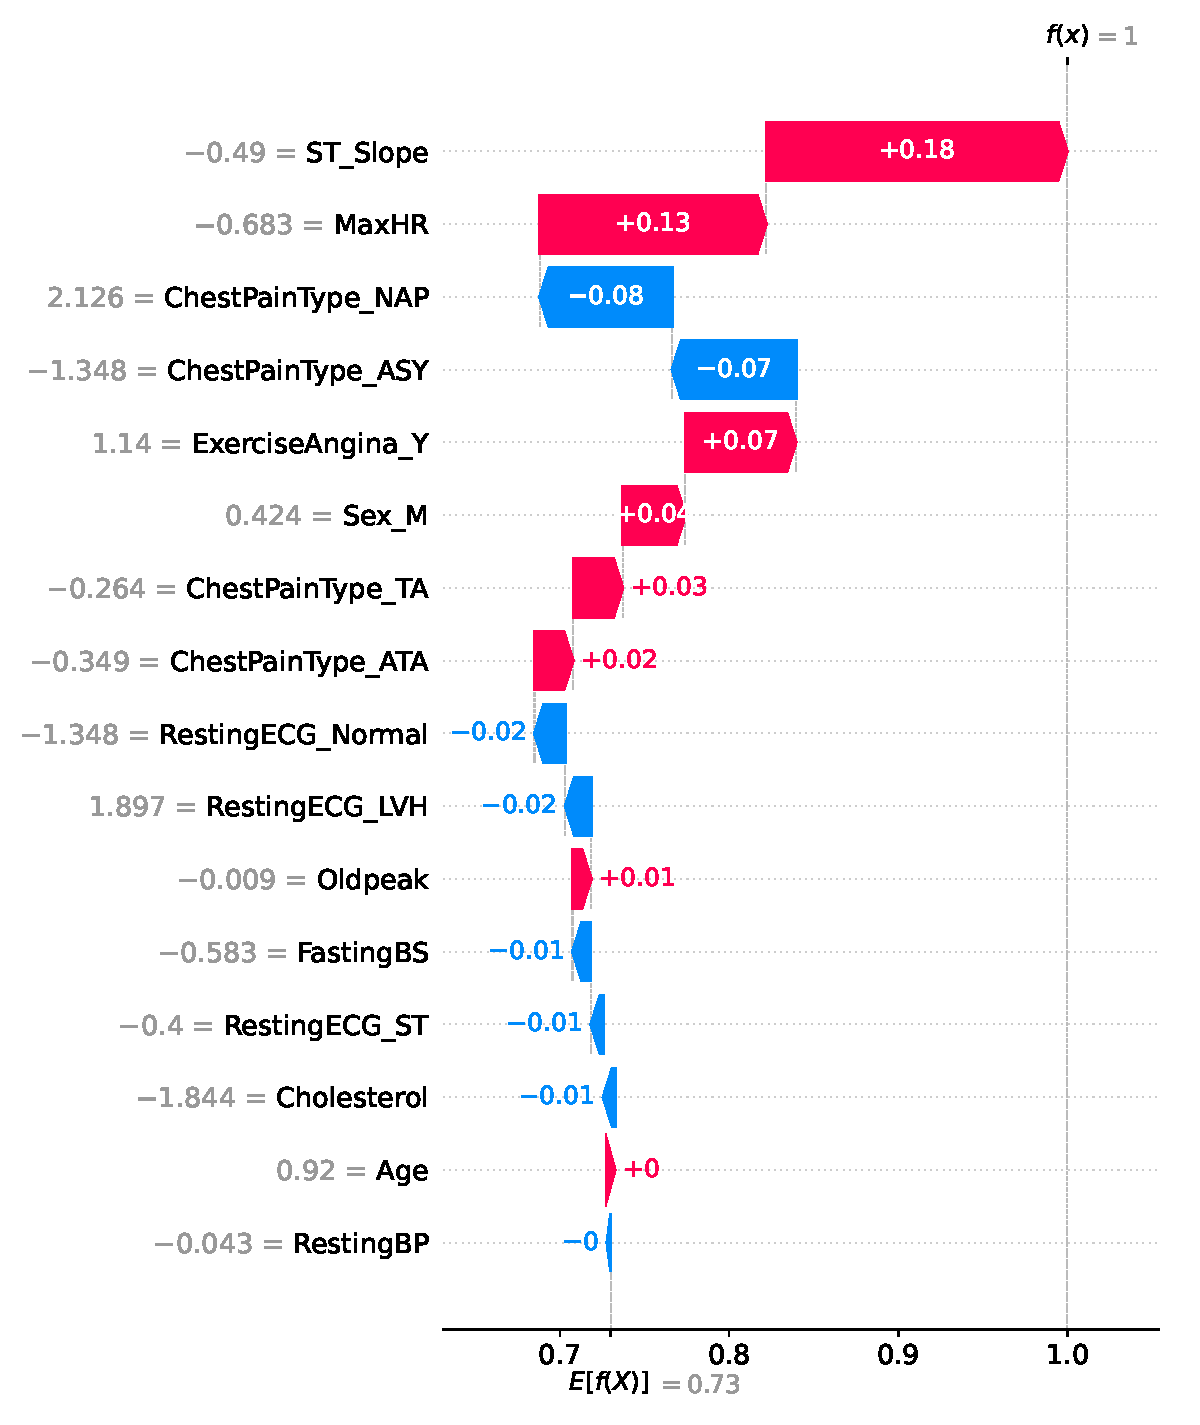
\includegraphics[width=1\textwidth]{images/shap_sample_positive_1.pdf}
        \caption{}
        \label{fig:shap_sample_positive_1}
    \end{subfigure}
    \begin{subfigure}{1\columnwidth}
        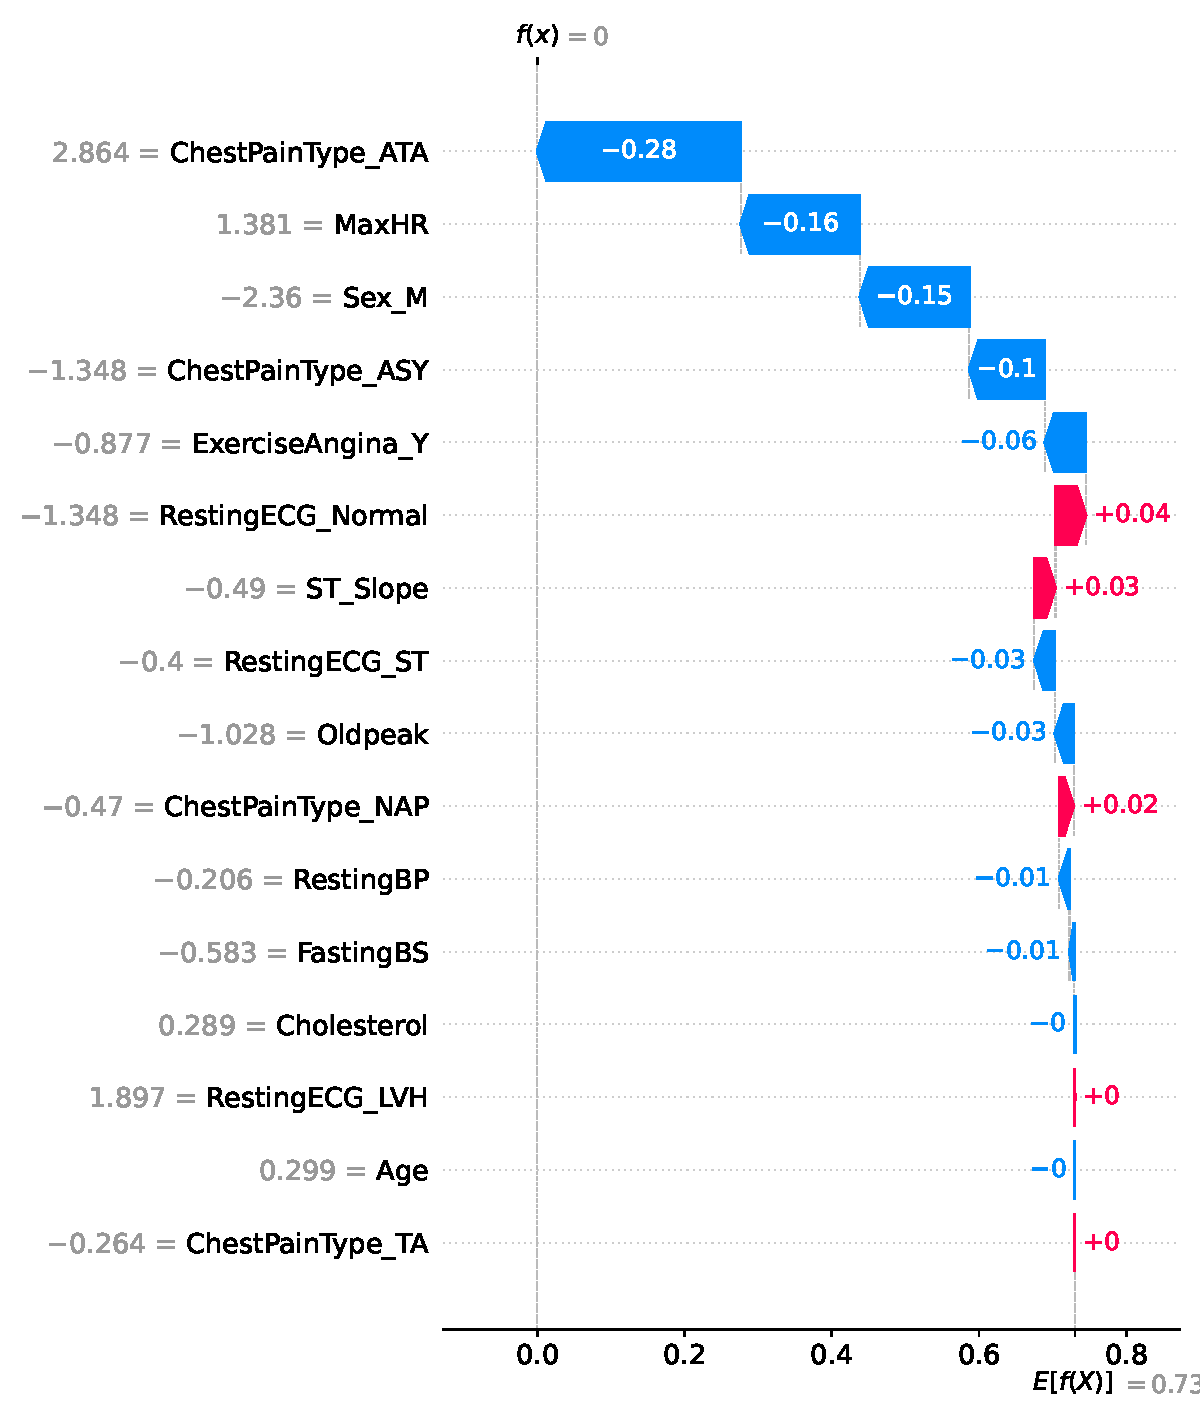
\includegraphics[width=1\textwidth]{images/shap_sample_positive_2.pdf}
        \caption{}
        \label{fig:shap_sample_positive_2}
    \end{subfigure}
    \begin{subfigure}{1\columnwidth}
        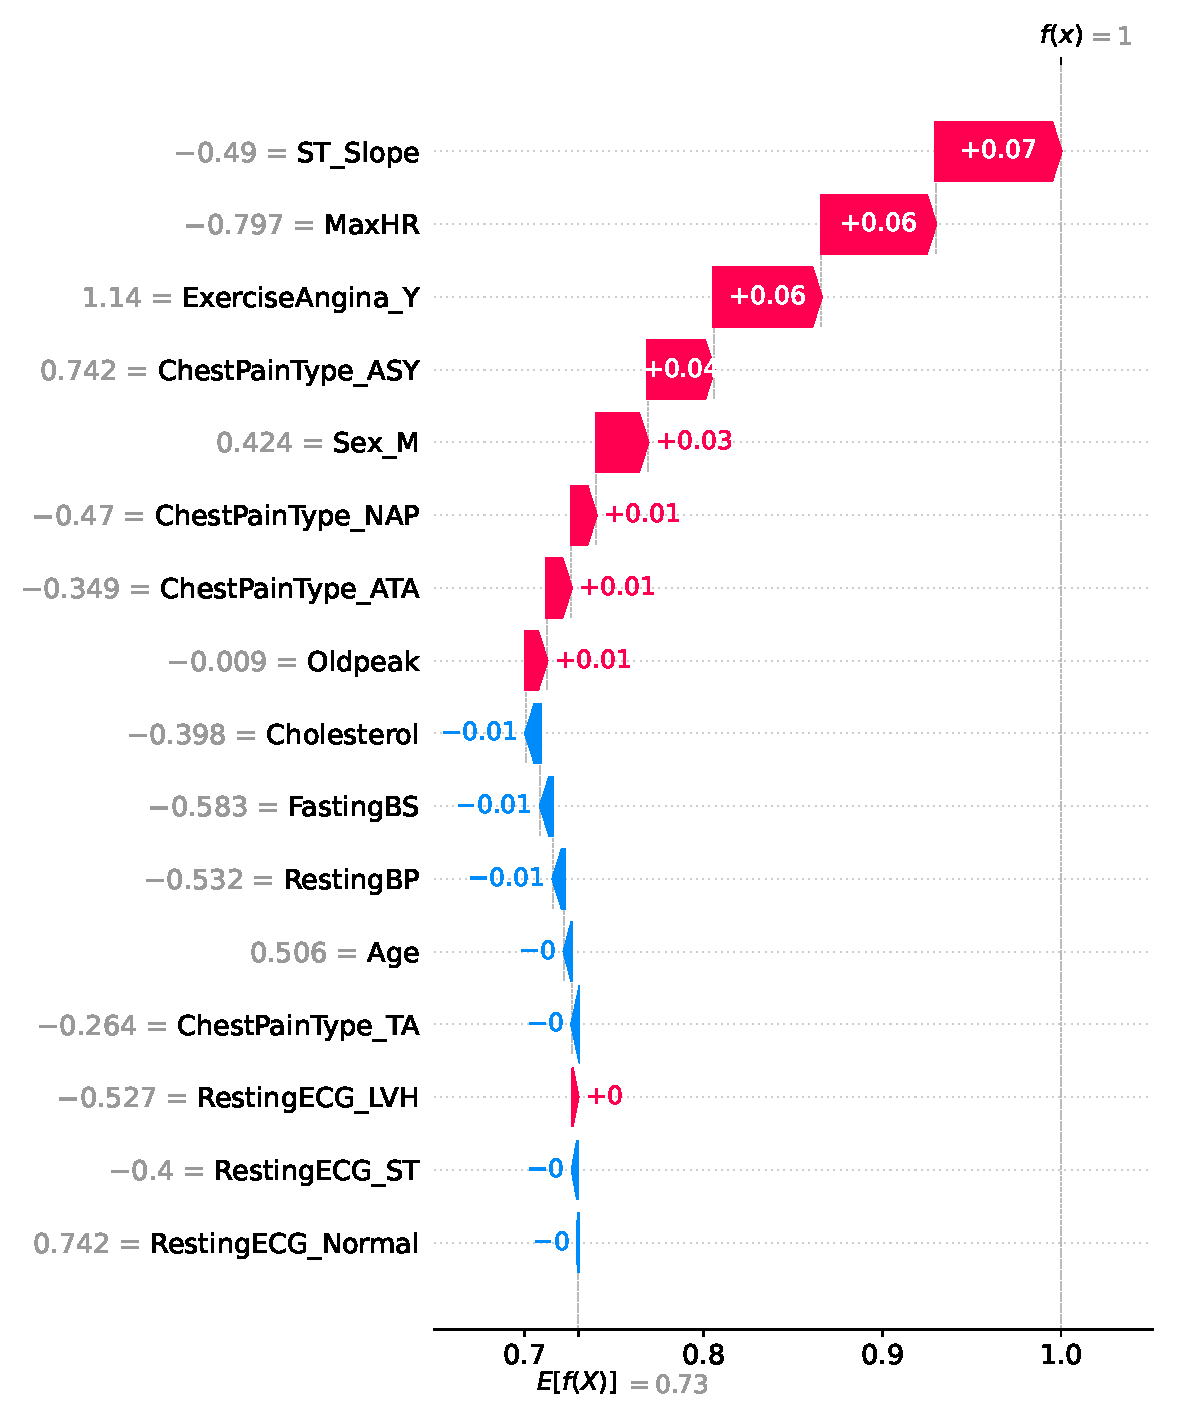
\includegraphics[width=1\textwidth]{images/shap_sample_positive_3.pdf}
        \caption{}
    \end{subfigure}
    \begin{subfigure}{1\columnwidth}
        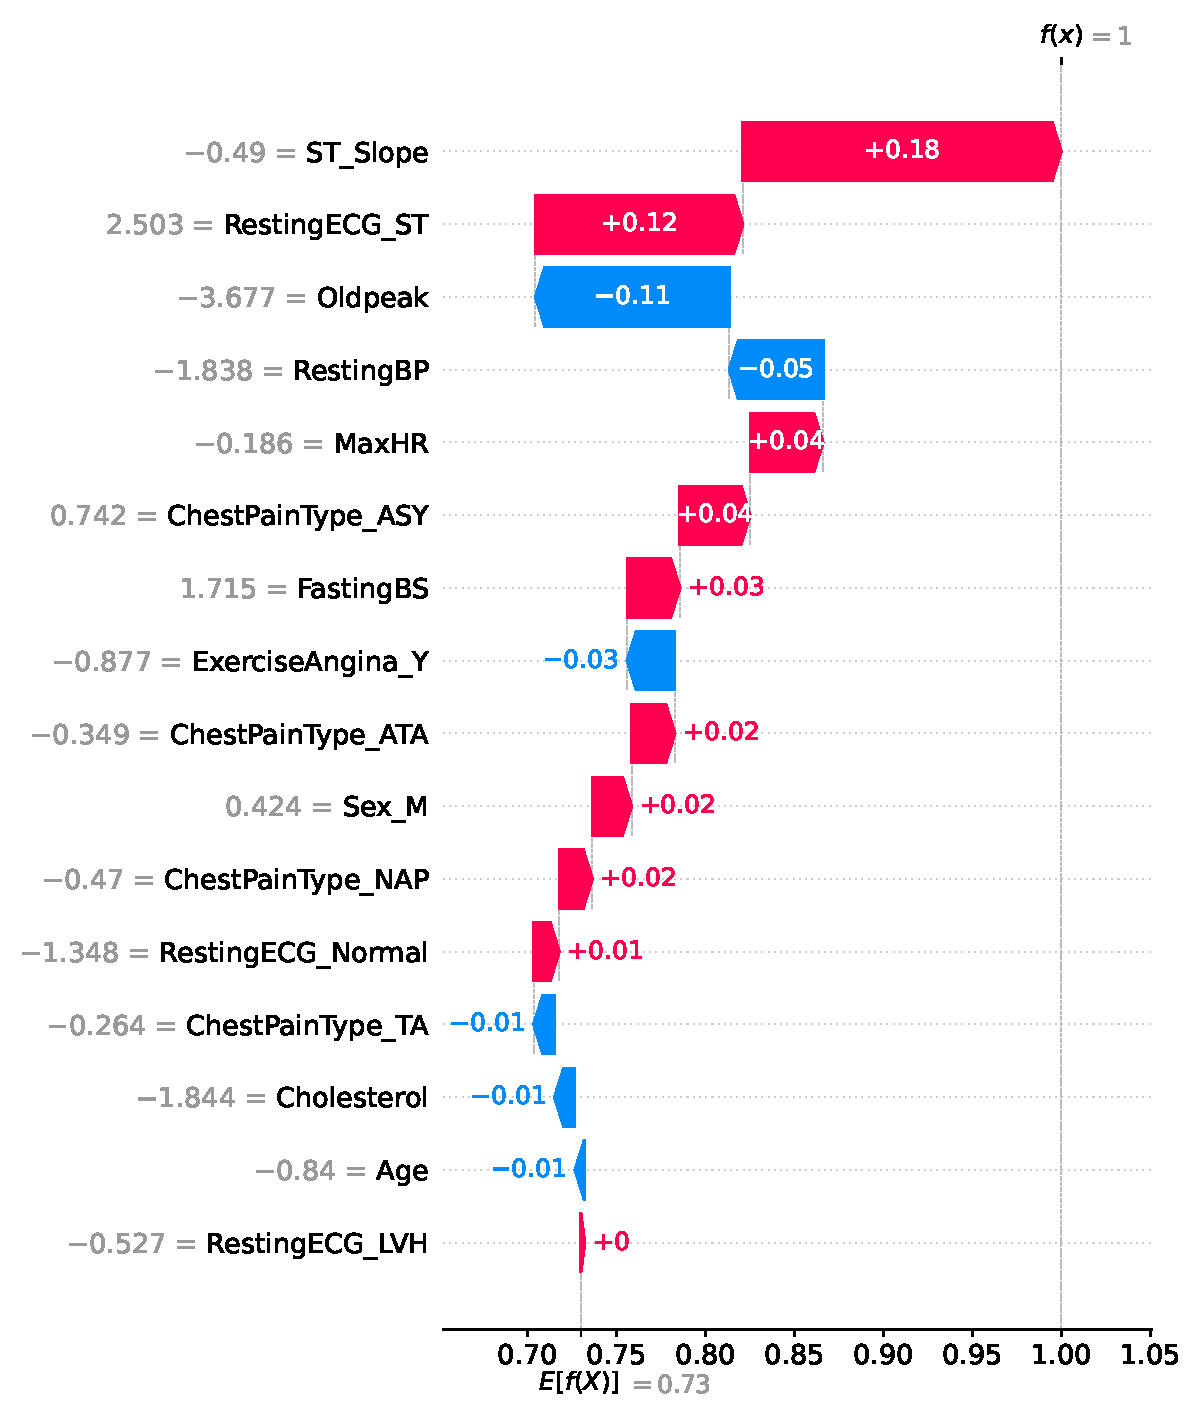
\includegraphics[width=1\textwidth]{images/shap_sample_positive_4.pdf}
        \caption{}
    \end{subfigure}
    \caption{Vizualization of SHAP explanations of the output of four \textbf{positive} samples from the test dataset. Features were normalized prior to calculating the Shapley values, as reflected in the displayed values of the samples. Note that sample in \protect\subref{fig:shap_sample_positive_2} has been misclassified as negative.}
    \label{fig:shap_sample_positive}
\end{figure*}
\begin{figure*}
    \centering
    \begin{subfigure}{1\columnwidth}
        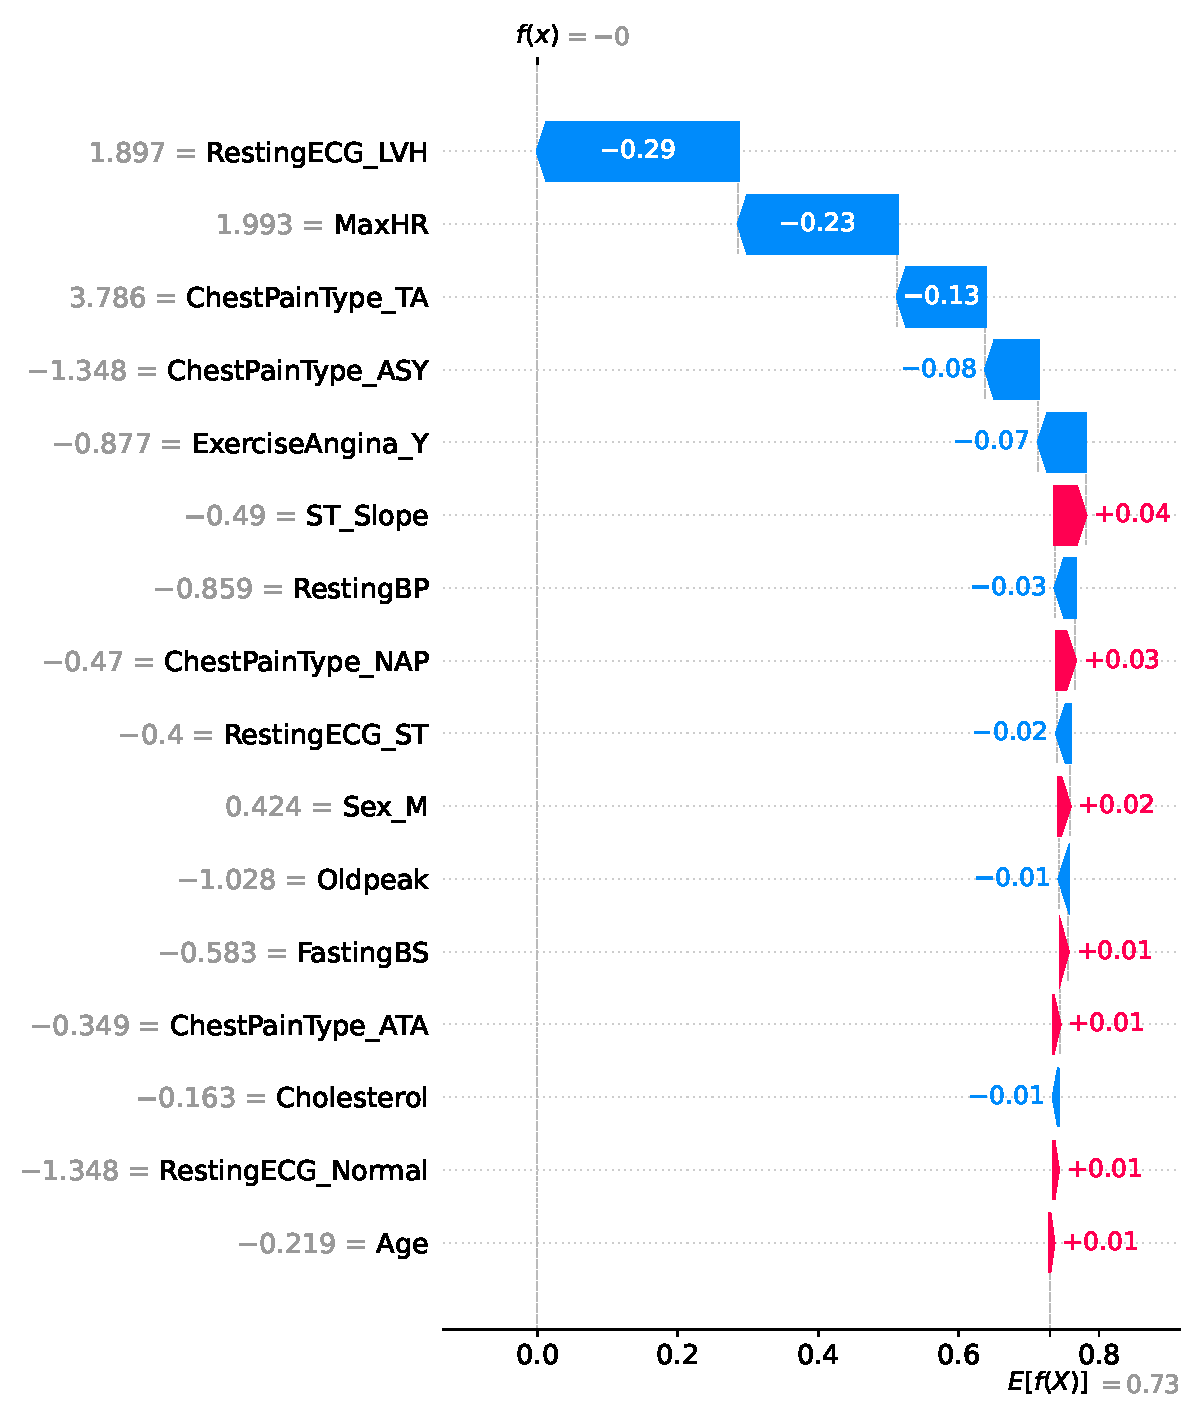
\includegraphics[width=1\textwidth]{images/shap_sample_negative_1.pdf}
        \caption{}
    \end{subfigure}
    \begin{subfigure}{1\columnwidth}
        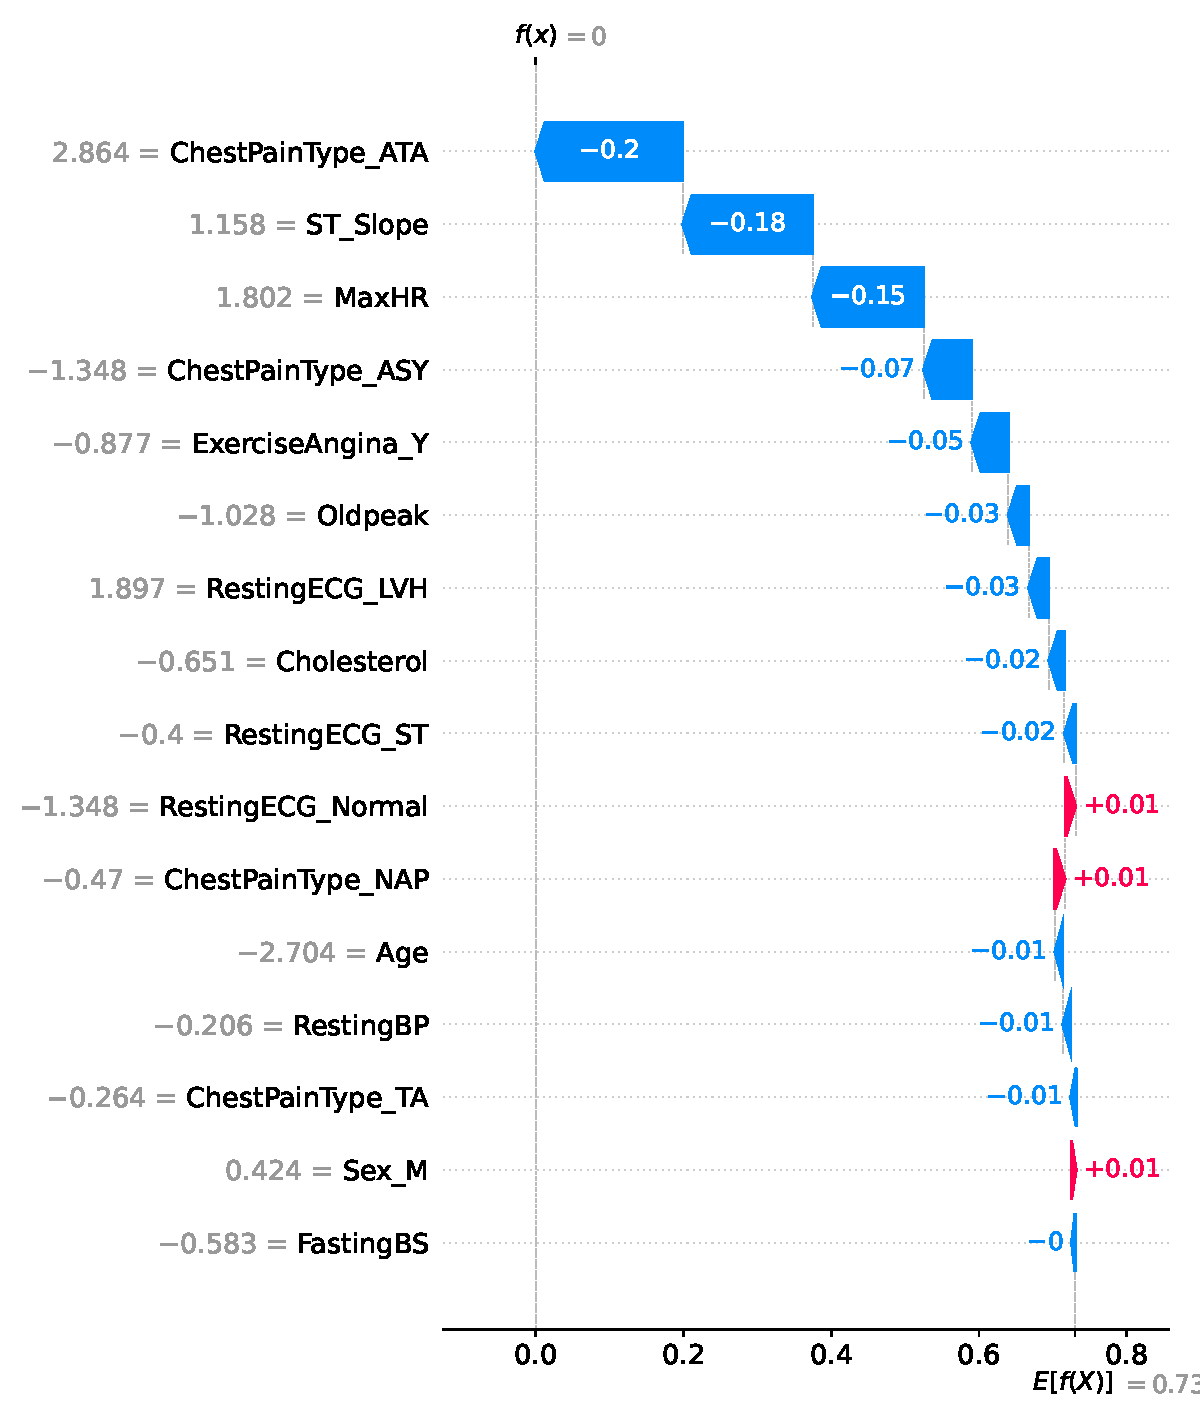
\includegraphics[width=1\textwidth]{images/shap_sample_negative_2.pdf}
        \caption{}
    \end{subfigure}
    \begin{subfigure}{1\columnwidth}
        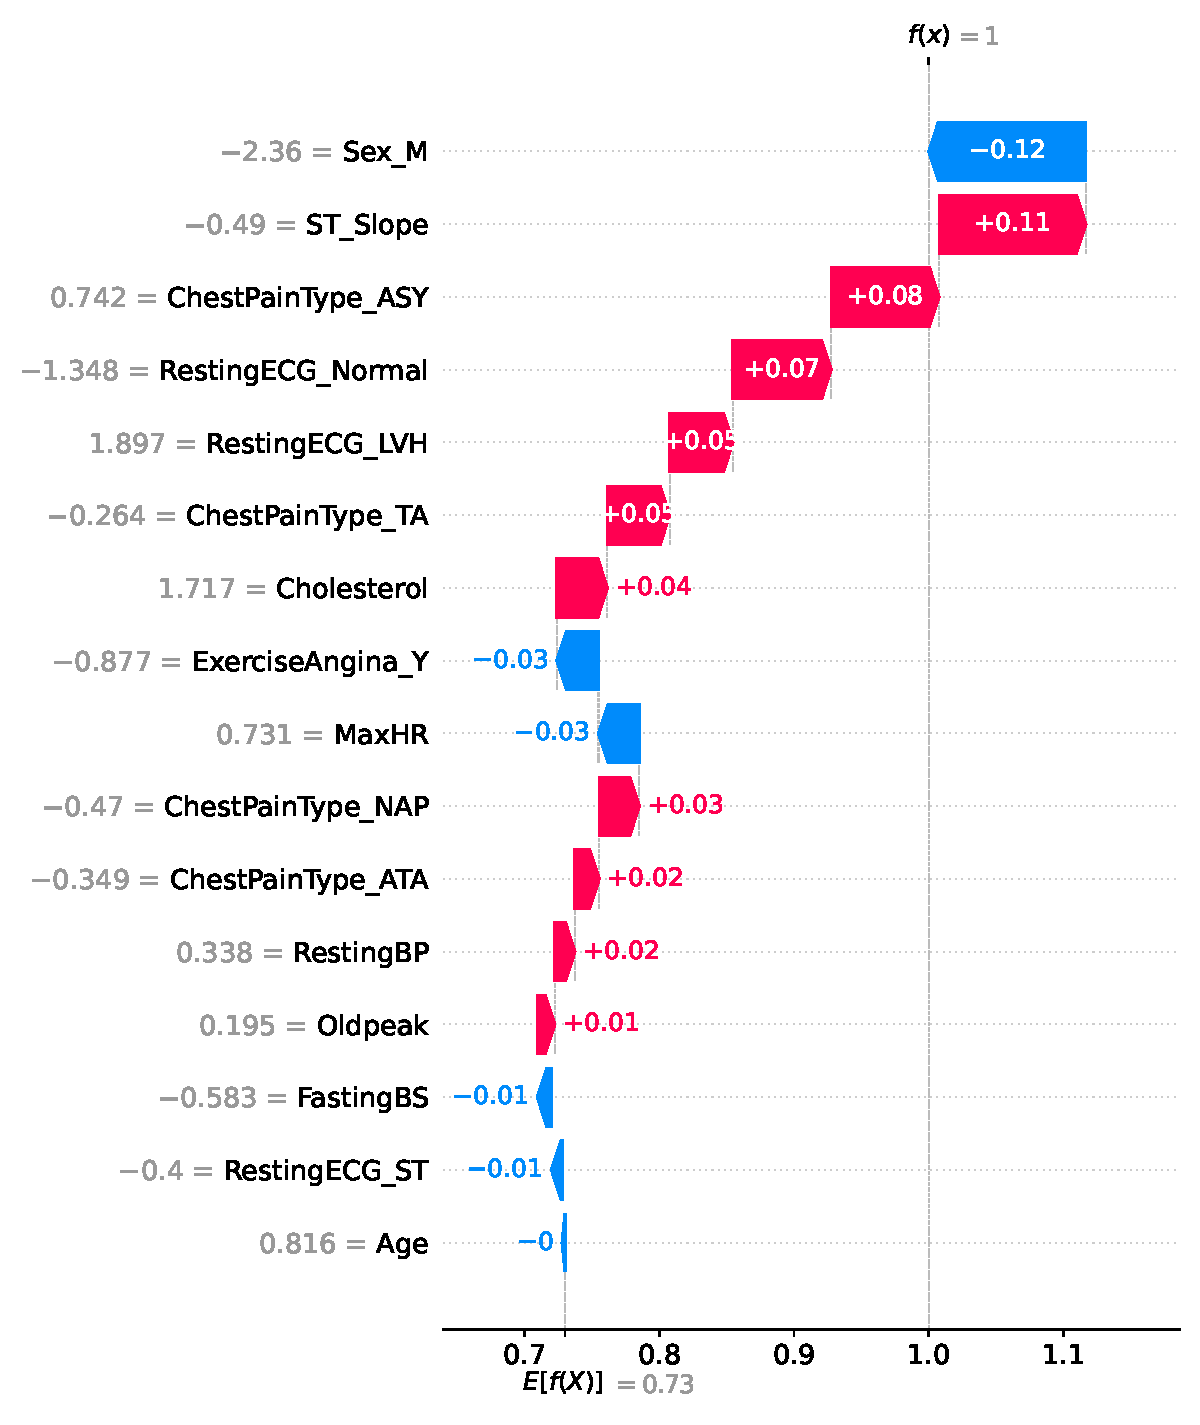
\includegraphics[width=1\textwidth]{images/shap_sample_negative_3.pdf}
        \caption{}
        \label{fig:shap_sample_negative_3}
    \end{subfigure}
    \begin{subfigure}{1\columnwidth}
        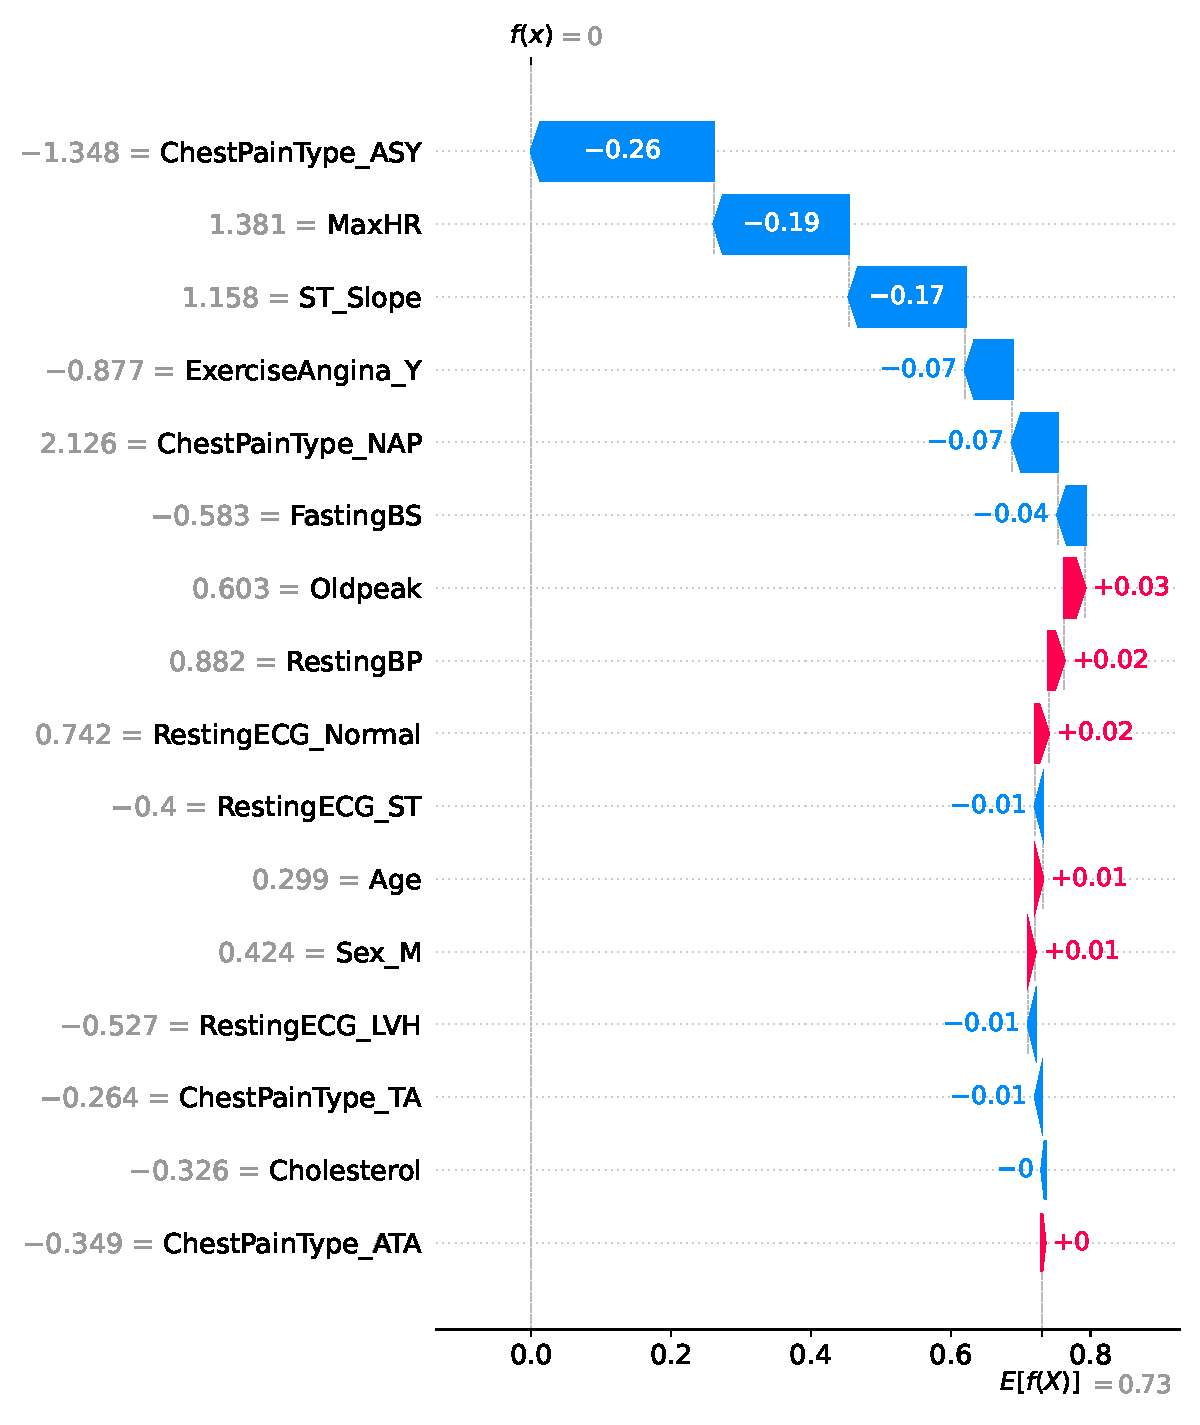
\includegraphics[width=1\textwidth]{images/shap_sample_negative_4.pdf}
        \caption{}
    \end{subfigure}
    \caption{Vizualization of SHAP explanations of the output of four \textbf{negative} samples from the test dataset. Features were normalized prior to calculating the Shapley values, as reflected in the displayed values of the samples. Note that the sample in \protect\subref{fig:shap_sample_negative_3} has been misclassified as positive.}
    \label{fig:shap_sample_negative}
\end{figure*}

\section*{General Questions}

\subsection*{Q1: How consistent were the different interpretable/explainable methods? Did they find similar patterns?}

Overall, there are differences in the features marked as important by the different models and explainability frameworks. However, a common trait of the three models (Lasso regression, Decision trees, MLP) is that all rank the two features \texttt{ST\_Slope} and \texttt{MaxHR} among the three most important features. Importances of other relatively important features are also correlated among the three models.

\subsection*{Q2: Given the “interpretable” or “explainable” results of one of the models, how would you explain and present them to a broad audience? Pick one example per part of the project.}
Let's look at the \autoref{fig:shap_sample_positive_1}, which shows the influence of individual features on the prediction for the sample (which is a sample from the test dataset). Without knowing anything about the patient, the model's output would be the prior, which is $E[f(\overline{x})] = 0.71$. The diagram then explains, due to which features the prediction ends up being $f(x)=1$.

For each feature, we would like to answer the following question: how much would our prediction change if the feature was unavailable? We cannot answer this question directly, since the MLP model requires all features to be present. However, we simulate the unavailability of a feature by replacing its value for the sample with different values from the 'background dataset', which, in our case, is the training dataset.
This technique is called 'masking', where values of each sample are masked by being replaced with other values from the training dataset.
Finally, the features (rows) are ordered by their individual contribution to the prediction for the sample.

In our solution we used the exact explainer, which completely enumerates the space of masking patterns and thus has exponential complexity in the number of features. However, many approximation algorithms exist which are suitable for larger datasets.


\subsection*{Q3: Did you encounter a tradeoff between accuracy and interpretability/explainability?}
Since for the MLP model, we used a model-agnostic feature importance explainer, the explainability of the model did not compete with its accuracy. Even if we preferred simpler explainability frameworks such as the Lasso regression or the Decision trees, this would not pose a direct tradeoff on the accuracy of the model, since all models achieved very similar F1 scores on the test dataset, between $79.2\%$ and $80.4\%$.

\subsection*{Q4: Do your findings from the interpretability/explainability methods align with the current medical knowledge about these diseases?}
It is well-founded in medicine that a patient is likely to have heart disease if the slope of the ST segment in their ECG diagram is other than flat, or if the maximum heart rate is too low.

\subsection*{Q5: If you had to deploy one of the methods in practice, which one would you choose and why?}
The SHAP explainability framework is, of those implemented in this project, the only model-agnostic, and thus most suitable in practice in general. However, for some specific classifier models, a different explainability framework might be more suitable. For example, if the classifier is a single decision tree, it is reasonable to explain the decision directly from the decision tree structure.


\clearpage

\setcounter{section}{0}
\section*{\large PART 2: PNEUMONIA PREDICTION}
\section{Exploratory Data Analysis}

For part 2 of the project, we use the Chest X-ray Images (Pneumonia) dataset from \cite{Kermany2018-ms}, which contains 5863 X-ray images of children aged 1-5, divided into two classes (pneumonia vs. normal). The majority (n=$3875$) of the images belong to class 'pneumonia', while relatively few images (n=$1341$) are from children without lung infection. This points to a major class imbalance, which we will take into account later on when training the CNN.

\subsection{Data Visualization}

We visualize some of the images in Figure \ref{fig:samples} to better understand our data.

\begin{figure}[H]
    \centering
    \begin{subfigure}{\columnwidth}
        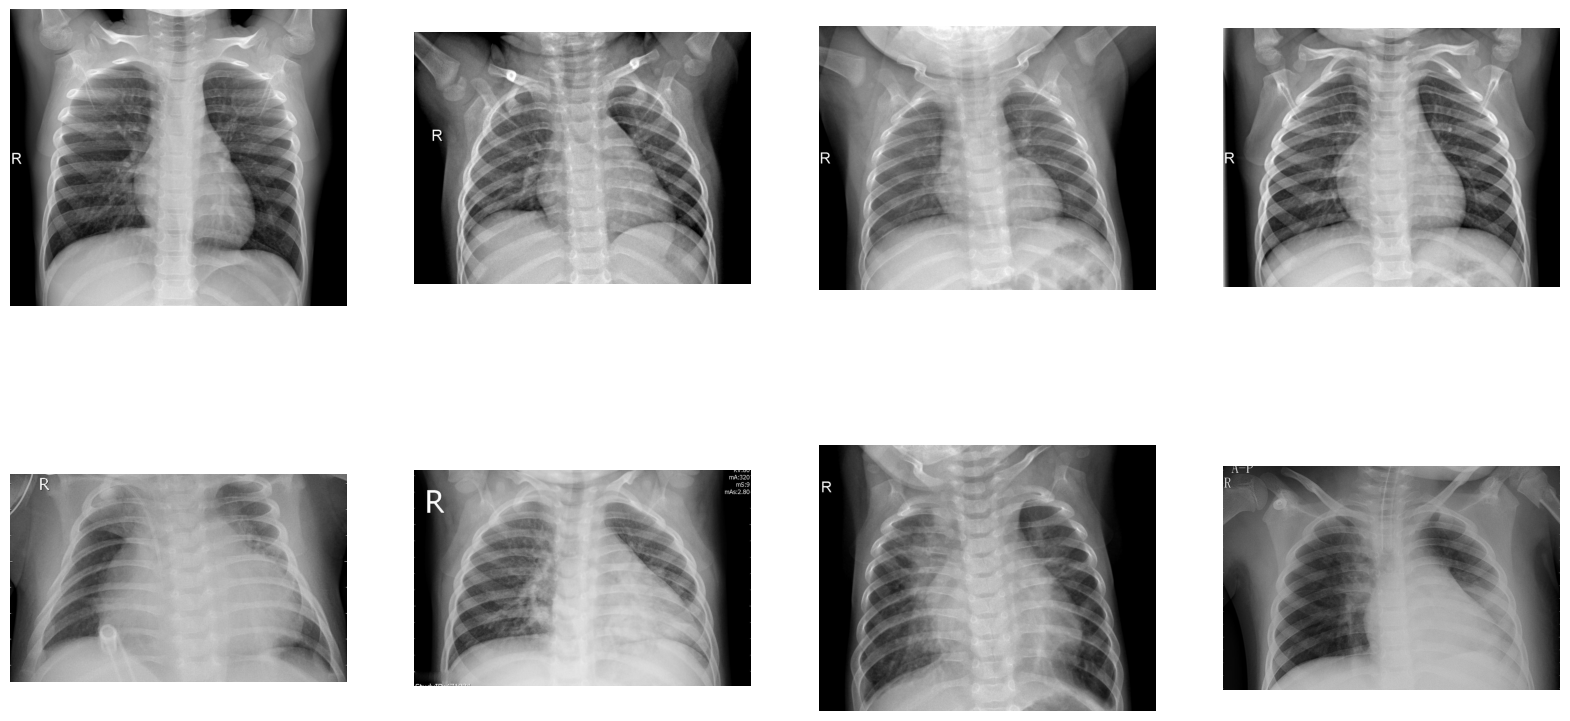
\includegraphics[width=1\textwidth]{images/samples.png}
    \end{subfigure}
    \caption{Visualization of X-rays from normal (upper row) and pneumonia (bottom row) class.}
    \label{fig:samples}
\end{figure}
Clearly, the lungs of sick patients appear more opaque (oftentimes in an asymmetric way), while the lungs of healthy patients appear more transparent/black (and equally so on both sides). In addition, the airways seem more pronounced and visible in sick patients.

A first problem becomes apparent when looking at Figure \ref{fig:samples}: the input sizes of the images are inconsistent. In addition, although not immediately apparent, some images are saved in 3-dimensional format, while others are saved as 2-dimensional images. We take this into account in all subsequent tasks by simply averaging the RGB values into a single grayscale value.

\subsection{Data Exploration}
For further data exploration, we first plot the average contrast distribution of all images in a histogram, and compare the resulting histograms between both classes. We expect images classified as 'pneumonia' to obtain slightly more bright values, due to the previously mentioned increased opaqueness of the lungs.
In addition, since input sizes are not homogeneous, we extract the image sizes and check if these are consistent between the two classes.
Finally, we apply principal component analysis (PCA) and check for consistency between train, validation, and test set.
Note that we normalize the image intensity for each image in order to allow for proper comparison between the different contrast windows used in X-ray imaging.

\begin{figure}[H]
    \centering
    \begin{subfigure}{\columnwidth}
        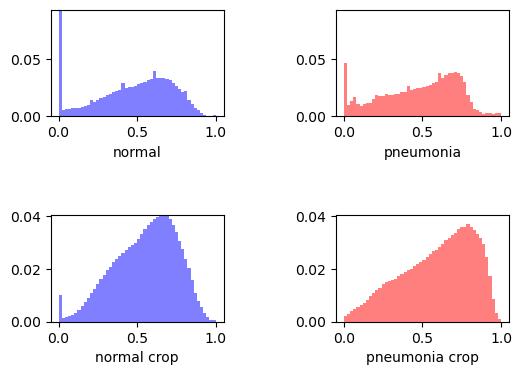
\includegraphics[width=1\textwidth]{images/histo_crop.png}
    \end{subfigure}
    \caption{Distribution of image intensities on a subset of cropped and non-cropped images.}
    \label{fig:histo_crop}
\end{figure}

\subsubsection{Histogram}
Due to the sheer size of some of the images, we check if cropping a subset of the images greatly affects the prominent features in the histogram. If not, we apply cropping for all further data analysis to prevent a needless increase in computation time.

As you can see in Figure \ref{fig:histo_crop}, although the histograms between cropped and non-cropped images are clearly different (the crop mostly removes black parts), the same trends can still be seen: the initial peak at intensity 0 (black) is higher in the normal samples, while the pneumonia samples show a peak at higher intensities than the normal samples. We deem these similarities to be important enough and therefore apply center-cropping to the images in all subsequent tasks.

\begin{figure}[H]
    \centering
    \begin{subfigure}{0.9\columnwidth}
        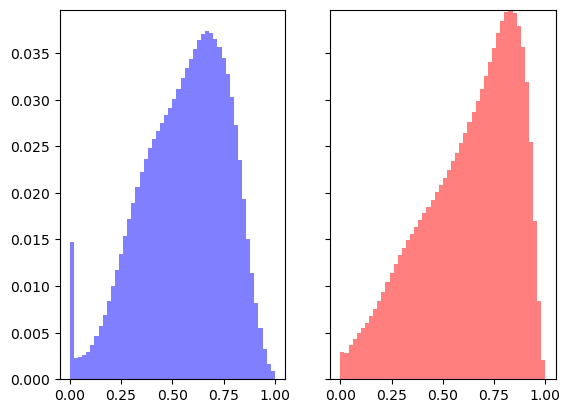
\includegraphics[width=1\textwidth]{images/histo.png}
    \end{subfigure}
    \caption{Distribution of image intensities over the entire dataset. Patients with pneumonia (red) have a peak at brighter values when compared to those without pneumonia (blue).}
    \label{fig:histo}
\end{figure}


If we now compare histograms obtained from the entire dataset, like in Figure \ref{fig:histo}, we can still see that samples with pneumonia seem to have brighter values in general, which makes sense, since one of the radiological features of pneumonia is an increase in visible tissue (visible due to inflammation and infection of the airways and lung parenchyma, but also due to fluid build ups) and the occurence of pleural effusions. Tissue and fluid are typically able to absorb more x-rays than air (which in contrast allows them to simply pass through), and therefore appear whiter on the X-ray image.

\subsubsection{Image Sizes}
Second, we visualize whether both classes have similar image sizes present. This might influence the cropping results (e.g. if all images in the 'normal' class have to be upsampled, while all images in the 'pneumonia' class should be downsampled, we might accidentally create a bias between the datasets).

\begin{figure}[H]
    \centering
    \begin{subfigure}{0.9\columnwidth}
        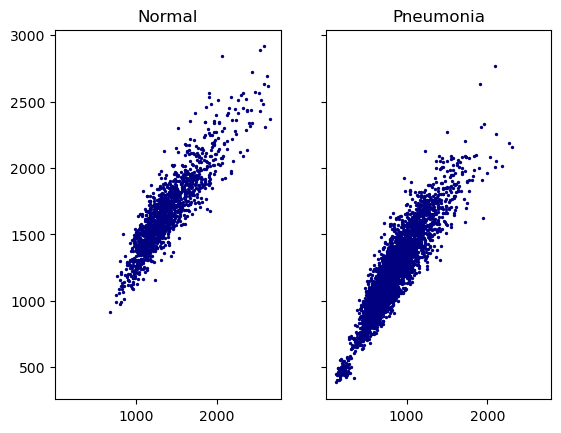
\includegraphics[width=1\textwidth]{images/sizes.png}
    \end{subfigure}
    \caption{Plot of image sizes per class. Height on y-axis, width on x-axis.}
    \label{fig:sizes}
\end{figure}

As can be seen in Figure \ref{fig:sizes}, image sizes vary widely, and images in the pneumonia class tend to have smaller sizes. We could make our model more robust to this by randomly zooming in/out on images and then resizing to the correct size. However, this could still cause a data bias, since images of patients with pneumonia will generally be zoomed into more if the size of the image is related to earlier cropping applied before adding the image to the dataset (and this seems to be the case). In addition, using the entire image as input for preprocessing will significantly decrease training speed. We therefore opt to only work with already center-cropped images.

\subsubsection{PCA}
Finally, we apply PCA to the cropped and normalized images in order to see whether there is a distinction between the two classes. We also compare with (but do not fit on) the validation and test set.

Figure \ref{fig:PCA} shows us that the main components are similarly distinct for train and test data, although there does seem to be more overlap for the test data.

\begin{figure*}
    \centering
    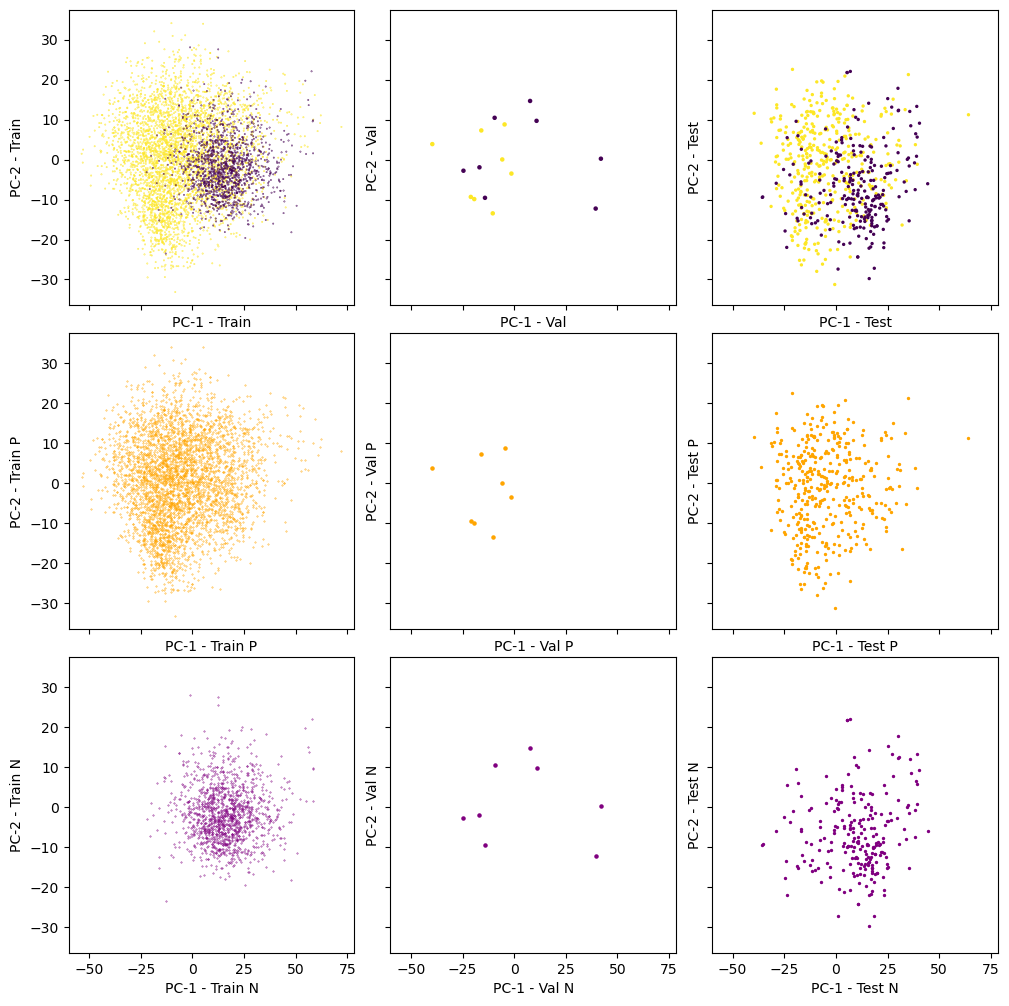
\includegraphics[width=0.8\textwidth]{images/PCA.png}
    \caption{Plot based on first two components of PCA. Upper row shows results for both classes in the same plot. Bottom two rows show them for each class separately. (orange: pneumonia, purple: normal).}
    \label{fig:PCA}
\end{figure*}

\section{CNN Classifier}

For our CNN, we first created a custom data generator class to allow resizing of the images using center cropping. We also save these images in a dataset for future use, to speed up training.
Second, we create a function able to convert our data to a dataframe in order to facilitate the use of the custom data generator. Note that we also add additional images ($2.5\%$ of the training set) from the training set to the validation set. Although some images appear to be obtained from the same patient, we did not make a distinction for this when dividing the train and validation data, but instead simply selected images at random.

\subsection*{A. Model Architecture}

We create a model similar to the model described in \cite{keras}, but with one dense layer less and with slightly different dropout ratios. This model has been used extensively in the Kaggle competition \cite{Kermany2018-ms} and has consistently produced good results. For additional data augmentation, we apply a random horizontal flip layer and a random rotation layer (limited to only small rotations).

\subsection*{B. Training}


We use an exponentially decaying learning rate, starting from $0.01$ with an overall decay rate of $0.96$ every 800 steps.
Since we work with images of two classes, binary crossentropy is used as loss function. In addition, we track how our model performs in terms of accuracy and precision/recall, the latter two especially useful in datasets with a class imbalance (like the dataset used in this project).

Note that we account for the class imbalance during training by using a larger weight for the smaller class (normal), and a smaller weight for the larger class (pneumonia). More specifically, we use the formula mentioned in \cite{tf}.

\subsection*{C. Evaluation}

We trained our model for 21 epochs, but used the checkpoint at 7 epochs for visualization in subsequent tasks, due to its clearer results.
Our 7-epoch model obtained an accuracy of around $90\%$ on the validation dataset, and $75\%$ on the test dataset.

When looking at the precision and recall of $0.77$ and $0.91$ respectively, we notice that the model outputs quite some false positives (i.e. we diagnose a patient with pneumonia when the patient is actually healthy), but relatively few false negatives. This, of course, is preferred behaviour, since we'd rather treat a healthy patient, instead of letting a sick patient (in the worst case) die.

Since our dataset is imbalanced, accuracy is not a very good measure. Technically, a model that outputs 1 (i.e. pneumonia) for every image could already get an accuracy of $62.5\%$ for the test dataset. Still, with an accuracy of around $75\%$, our model clearly performs better, which at the very least means that it has learnt some features related to healthy and sick patients.

\section{Integrated Gradients}


\begin{figure*}
    \centering
    \begin{subfigure}{\textwidth}
        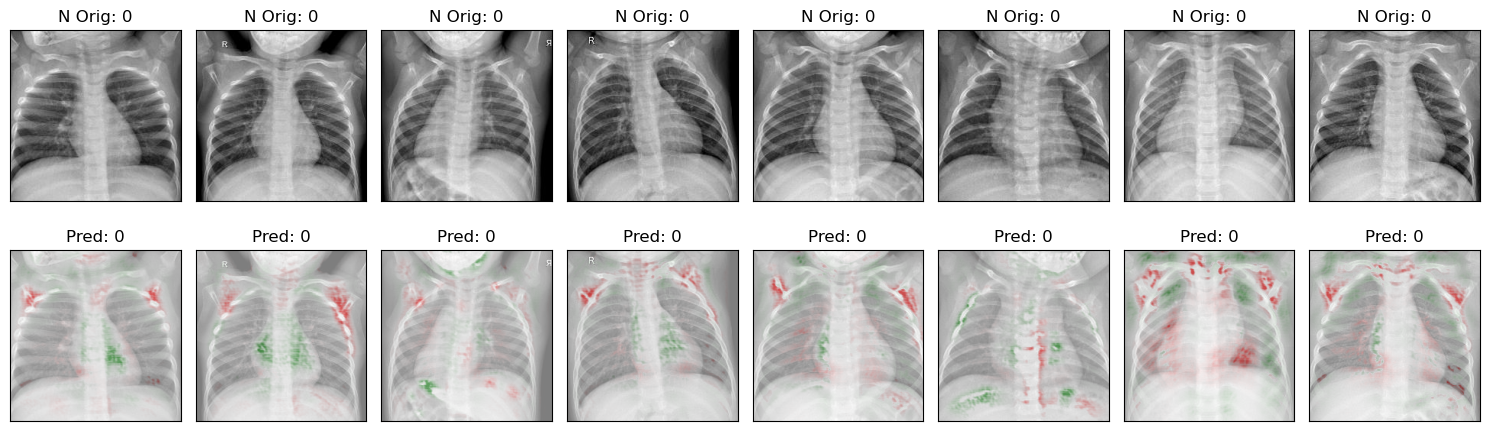
\includegraphics[width=1\textwidth]{images/IG_train.png}
    \end{subfigure}
    \centering
    \begin{subfigure}{\textwidth}
        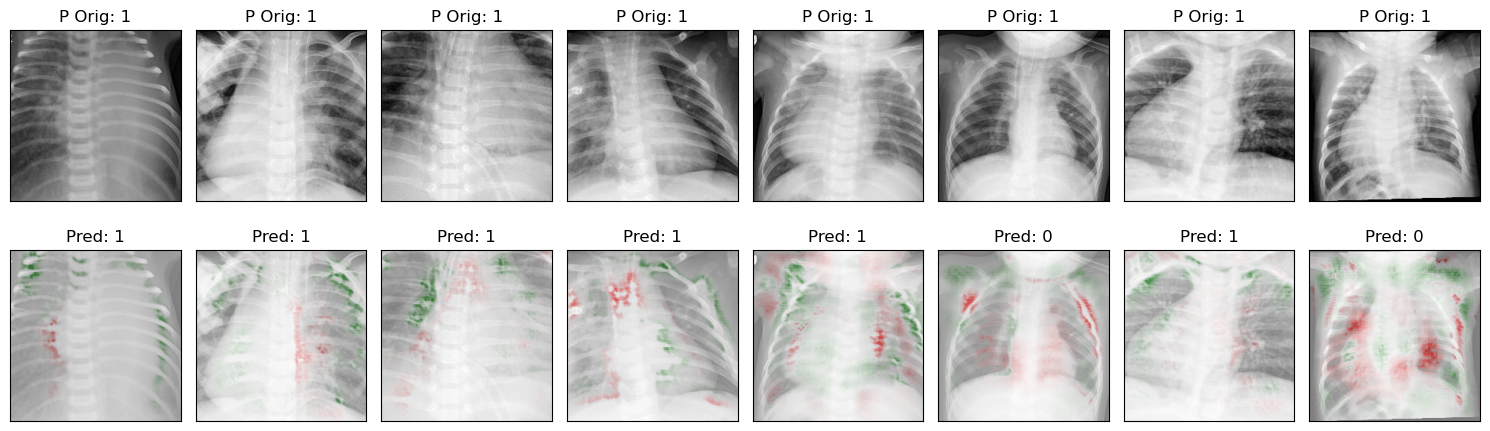
\includegraphics[width=1\textwidth]{images/IG_train_P.png}
    \end{subfigure}
    \caption{Training images to which integrated gradients was applied. Upper two rows are from healthy patients, bottom two rows from patients with pneumonia. The 1st and 3rd row contain the input image, the 2nd and 4th row contain an added overlay from integrated gradients. In red is the negative attribution, in green the positive attribution.}
    \label{fig:ig_train}
\end{figure*}

Integrated gradients (IG) applied to images allows us to attribute a certain importance to each pixel. This importance can be negative, i.e. this pixel makes the prediction for the class that is currently being looked at less likely, but also positive, i.e. this pixel positively contributes to the prediction of that class.

For applying the integrated gradients method, we adapt the code from \cite{alibi} and calculate the gradient along the path between the given image and a black 'baseline' image. We choose an all-zeros baseline image because the background of an X-ray image is also black, and signifies the 'absence of signal'. This is deemed important in the original paper from Sundararajan et al. \cite{ig}.

We use the trapezoidal version of Riemann gradient approximation, as this seems to be what \cite{ig} mentions.

\subsection*{A. Visualization}

As you can see in Figure \ref{fig:ig_train}, the main focus point for most patients, both healthy and sick, is the bones in the shoulder and the outer contours of the upper ribs. For healthy patients, this is considered a negative attribute, for sick patients a positive one.

In addition, some attention is paid to the areas where the airways branch out, near the center of the image (i.e. near the hilums of the lungs). This makes sense, since sick patients often have increased thickening of the smaller airways.

In some images, we are also able to observe focus on the spaces in between the ribs, which seems to be a sensible place to look, since that's where we can see the lungs and its contents the best.

The reason why the model seems to focus on the chin, might be due to its ability to look for enlarged lymph nodes in the throat area, since the pneumonia might have been preceded by a throat infection.

Overall, the model is focusing a lot on bones, but this could be contributed to the fact that the shoulders in healthy patients are often included in the X-ray, while this does not seem to happen as often for patients with pneumonia. Perhaps it was more difficult to keep a sick child still during the imaging, as compared to healthy children, and therefore the parents' help was needed to 'pin' the sick children down (maybe holding their head still with their hands), which caused the image to not include the lower part of the head and upper part of the shoulders. This is just a hypothesis of course.

The results for the test set in Figure \ref{fig:ig_test} largely confirm what is seen in the training data, although the shoulders seem to be detected more often for sick patients.

\begin{figure}
    \centering
    \begin{subfigure}{\columnwidth}
        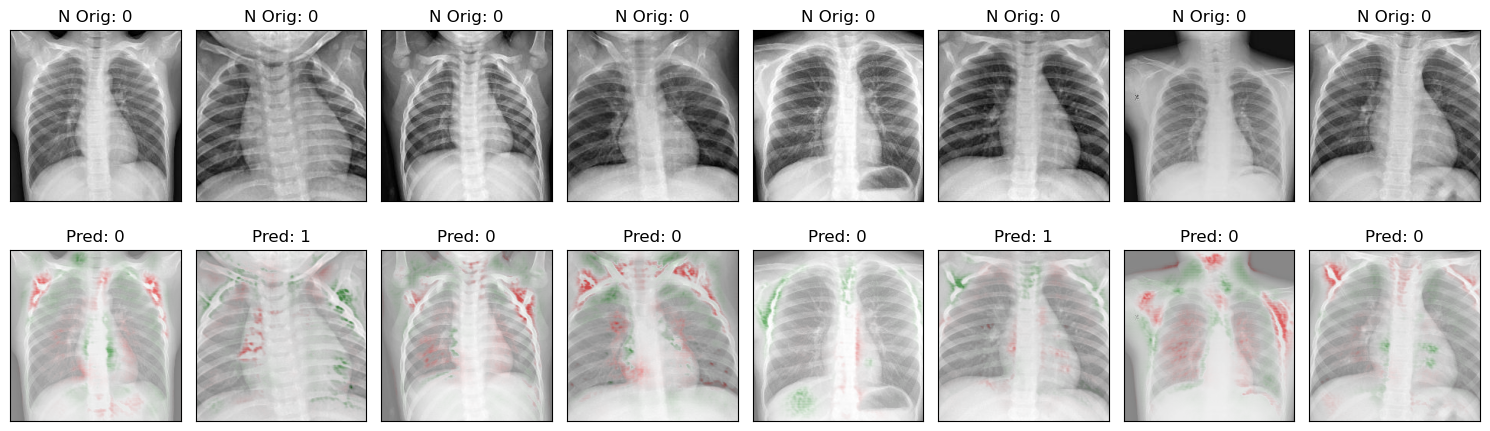
\includegraphics[width=1\textwidth]{images/IG_test.png}
    \end{subfigure}
    \centering
    \begin{subfigure}{\columnwidth}
        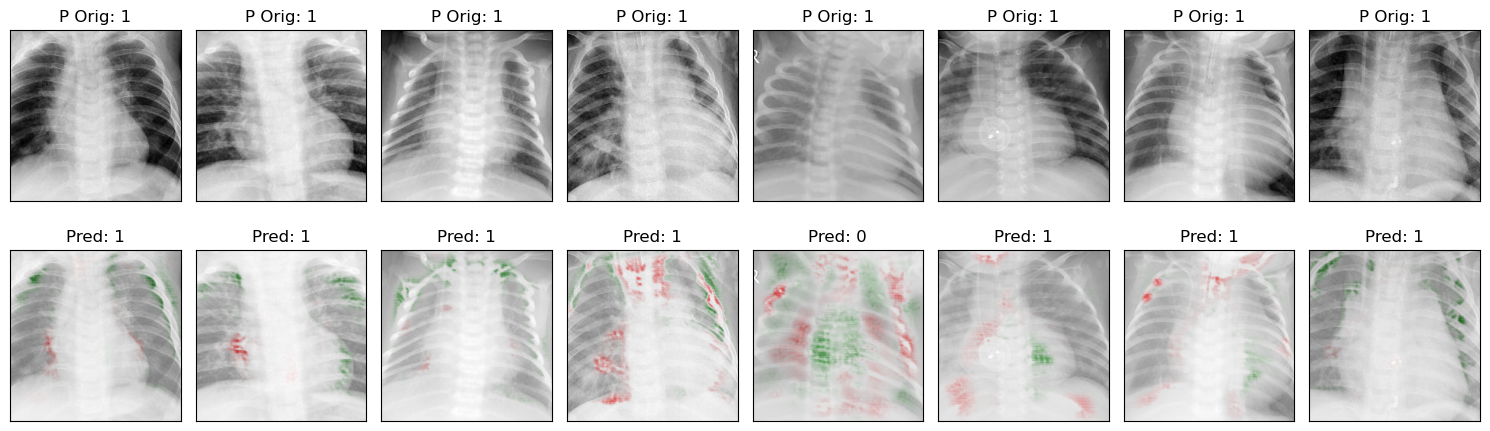
\includegraphics[width=1\textwidth]{images/IG_test_P.png}
    \end{subfigure}
    \caption{Test images to which integrated gradients was applied. Upper two rows are from healthy patients, bottom two rows from patients with pneumonia. The 1st and 3rd row contain the input image, the 2nd and 4th row contain an added overlay from integrated gradients. In red is the negative attribution, in green the positive attribution.}
    \label{fig:ig_test}
\end{figure}
\begin{figure*}
    \centering
    \begin{subfigure}{\textwidth}
        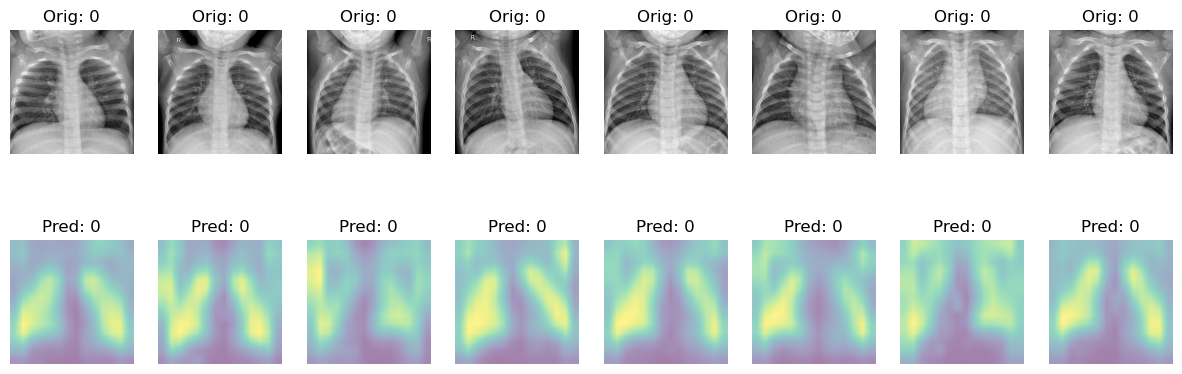
\includegraphics[width=1\textwidth]{images/gc_train.png}
    \end{subfigure}
    \centering
    \begin{subfigure}{\textwidth}
        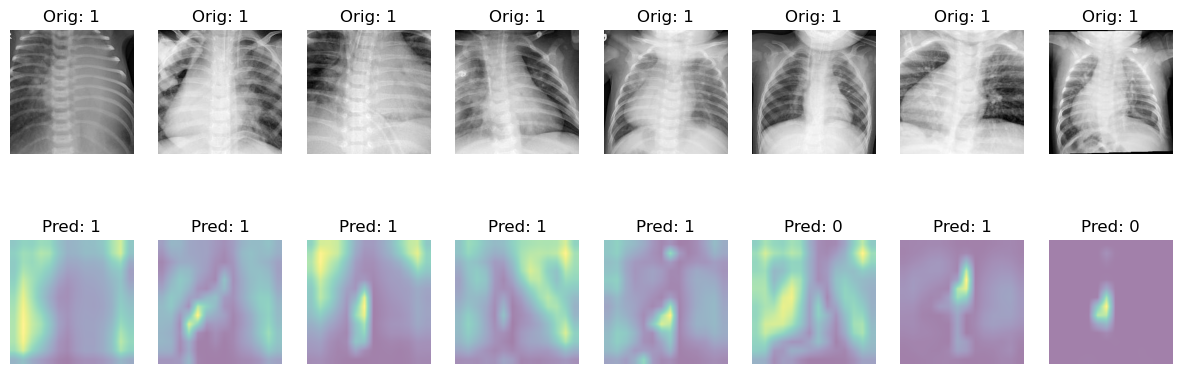
\includegraphics[width=1\textwidth]{images/gc_train_P.png}
    \end{subfigure}
    \caption{Training images to which Grad-CAM was applied. Upper two rows are from healthy patients, bottom two rows from patients with pneumonia. The 1st and 3rd row contain the input image, the 2nd and 4th row contain the overlay produced by Grad-CAM. Yellow signifies the highest attribution, purple the lowest attribution.}
    \label{fig:gc_train}
\end{figure*}

\section{Grad-CAM}

Grad-CAM is a method that highlights parts of an image based on the contribution of the respective neurons for class prediction. For this, Grad-CAM uses gradients between the last convolutional layer and the decisions of the output layer.
For our implementation, we modify the code from \cite{gradcam}.

\subsection*{A. Visualization}
If we look at the results on the training dataset in Figure \ref{fig:gc_train}, the pattern in healthy patients is very consistent, with the main focus on the lungs, and little focus on everything below the diaphragm. In addition, the hilum of the lungs (where the airways 'enter' the lungs) is also represented well, but this is partially 'masked out' due to the many overlapping structures nearby, such as the heart and the vertebra.

The model does not explain finer details due to the fact that Grad-CAM only produces a coarse localization map.

For sick patients, both global and local importance can be seen, the global focus on the lungs similar to healthy patients (albeit sometimes absent).

\begin{figure}
    \centering
    \begin{subfigure}{\columnwidth}
        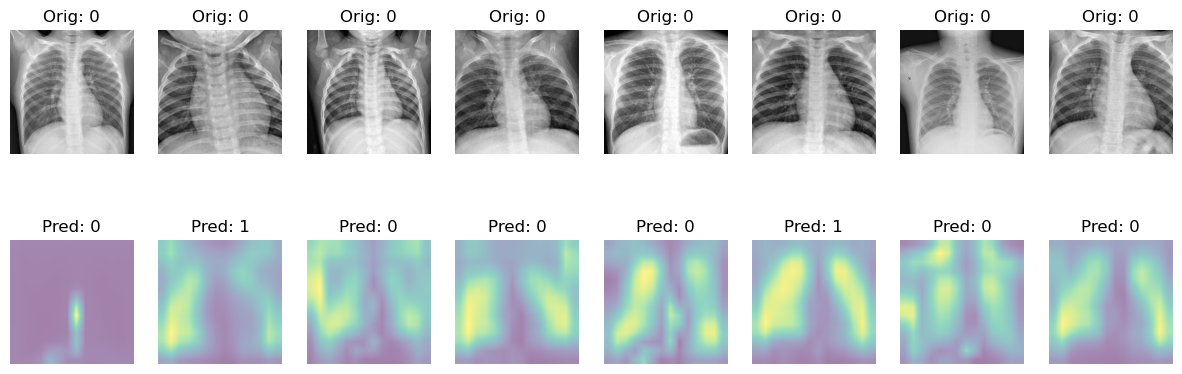
\includegraphics[width=1\textwidth]{images/gc_test.png}
    \end{subfigure}
    \centering
    \begin{subfigure}{\columnwidth}
        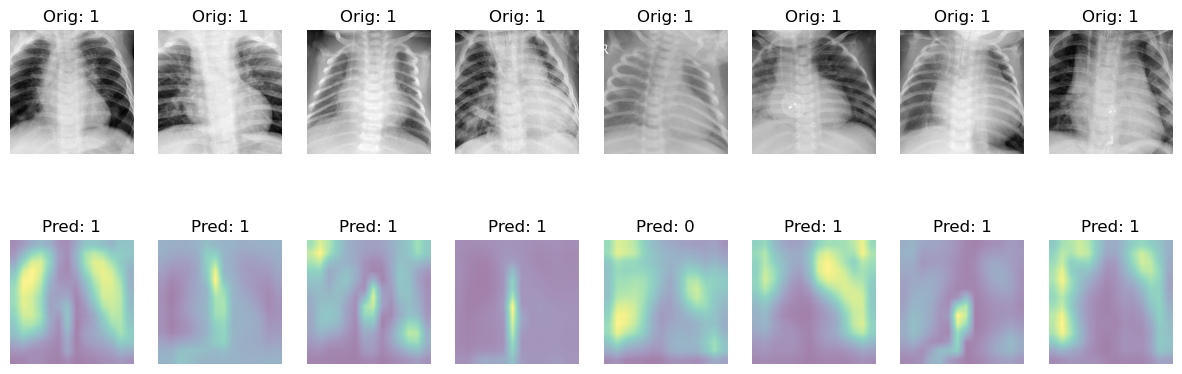
\includegraphics[width=1\textwidth]{images/gc_test_P.png}
    \end{subfigure}
    \caption{Test images to which Grad-CAM was applied. Upper two rows are from healthy patients, bottom two rows from patients with pneumonia. The 1st and 3rd row contain the input image, the 2nd and 4th row contain the overlay produced by Grad-CAM. Yellow signifies the highest attribution, purple the lowest attribution.}
    \label{fig:gc_test}
\end{figure}

The local importance at the vertebra seems a bit odd, although there might be some enlarged lymph nodes there. An alternative hypothesis is that the patient might have a feeding tube in place, which would make sense, as sick children often refuse to eat food. An additional contributing factor might be that the images from the healthy patients are more similar to one another, both in positioning of the child andin terms of radiological findings, while sick children with many different radiological findings are more difficult to keep in a fixed position during imaging.

All in all, we can conclude that the model knows that the lungs are the most important part of the X-ray image that contributes to the final prediction, but is still sometimes confused by the intra-class differences of sick patients.

All previously mentioned patterns can also be seen in images in the test set in Figure \ref{fig:gc_test}.
\section{Data Randomization Test}

\begin{figure*}
    \centering
    \begin{subfigure}{\textwidth}
        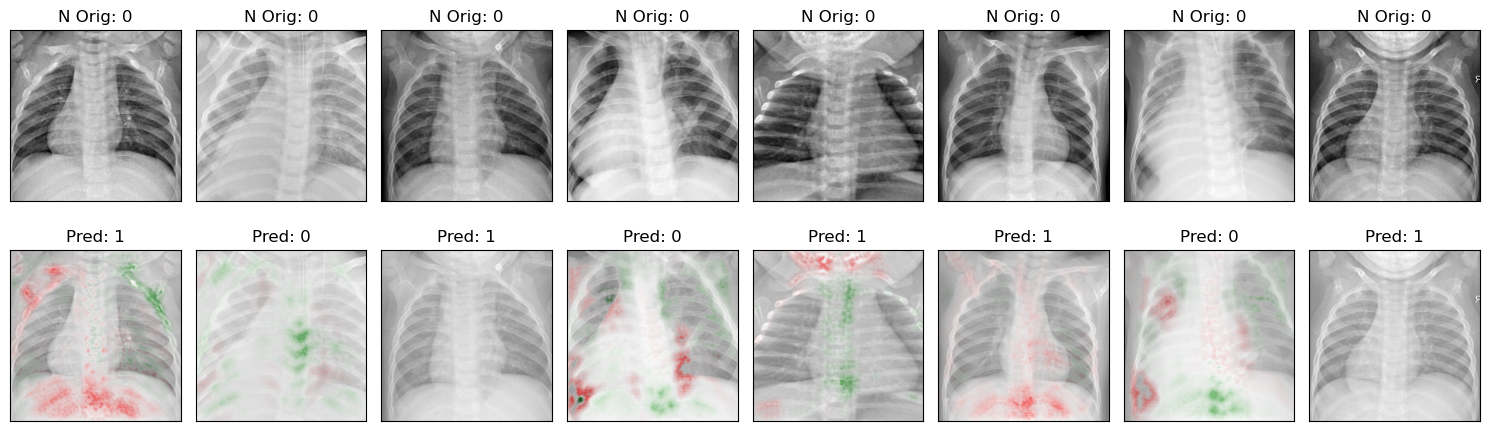
\includegraphics[width=1\textwidth]{images/ig_rand_train.png}
    \end{subfigure}
    \centering
    \begin{subfigure}{\textwidth}
        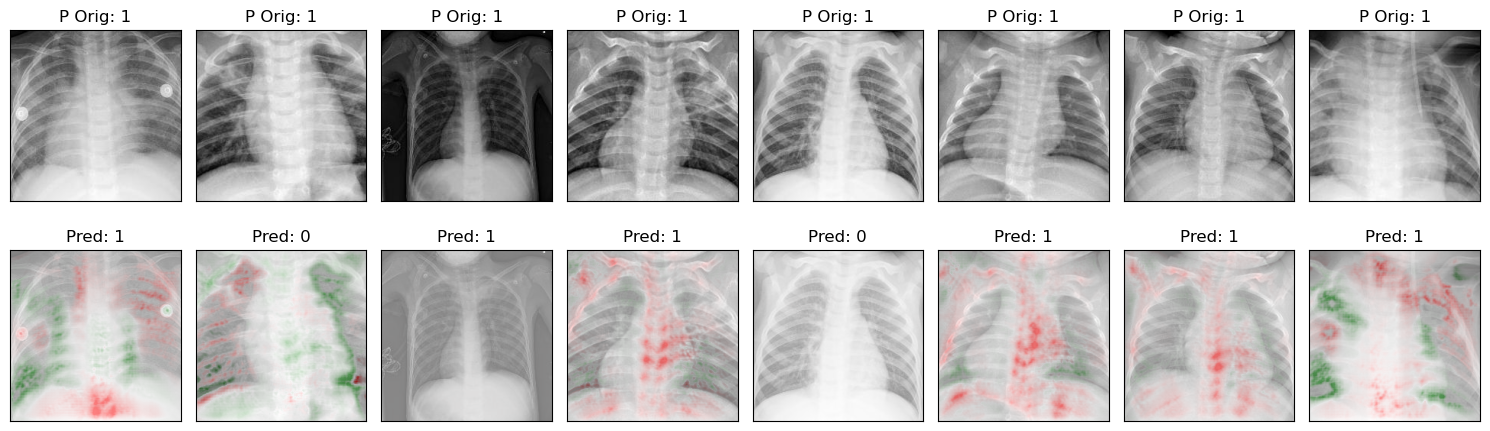
\includegraphics[width=1\textwidth]{images/ig_rand_train_P.png}
    \end{subfigure}
    \caption{Training images to which integrated gradients was applied. The model was finetuned on random labels. Upper two rows are from healthy patients, bottom two rows from patients with pneumonia. The 1st and 3rd row contain the input image, the 2nd and 4th row contain an added overlay from integrated gradients. In red is the negative attribution, in green the positive attribution.}
    \label{fig:ig_rand_train}
\end{figure*}

For the data randomization test, we train our model with random labels to ensure it isn't just a fancy edge detector.

We tried two approaches. First, we tried to train a model from scratch, with the same settings and parameters as before, but with randomized labels. We trained for many epochs (50 in total), but at no point was the model able to learn something useful, and applying Grad-CAM or integrated gradients only resulted in an empty overlay. This of course meant that our initial model was able to learn relevant information from the X-ray images.

Still, to allow for better visualization, we tried a second approach: we fine-tuned our model for 16 epochs on random labels, after pre-training on the true labels for 7 epochs. The fine-tuning was stopped when the variance of the predicted results was near 0, which coincided with the end of epoch 16. This was to ensure that the model was not too confident in its predictions.
The accuracy on the test set was, as expected, around 50\%. Precision and recall also had values close to 0.5.

\subsection*{A. Integrated Gradients}

For integrated gradients, there seems to be an increased focus on bone tissue, similar to what we observed when training on true labels, but this time, it is likely due to the sensitivity of the model to white areas. For example, in Figure \ref{fig:ig_rand_train} some images highlight the ribs itself instead of the area of lung tissue in between. In addition, the border of the heart is marked more clearly than before.

\begin{figure}
    \centering
    \begin{subfigure}{\columnwidth}
        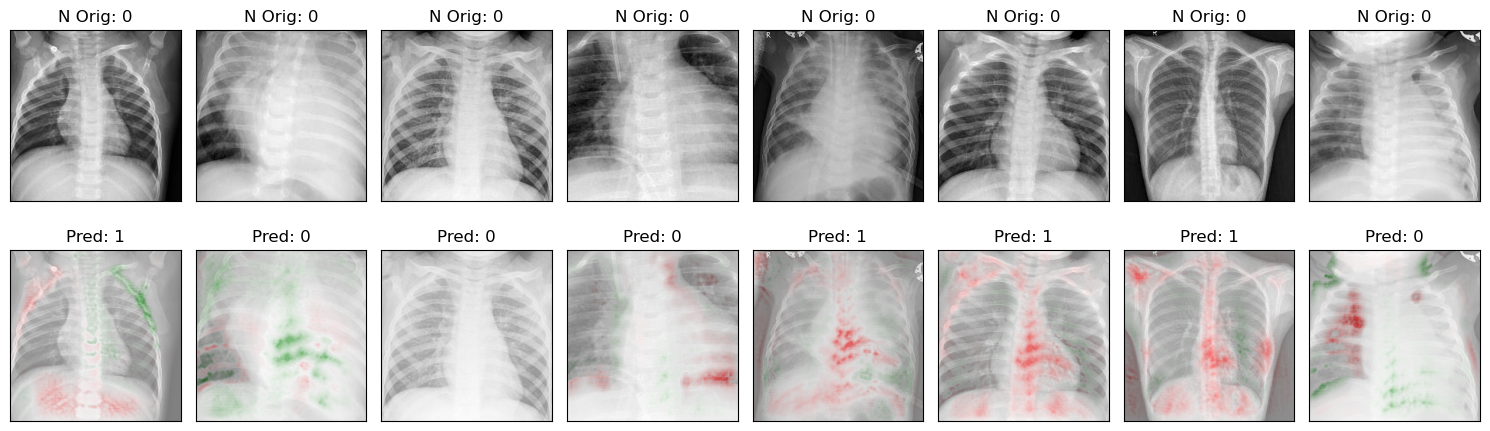
\includegraphics[width=1\textwidth]{images/ig_rand_test.png}
    \end{subfigure}
    \centering
    \begin{subfigure}{\columnwidth}
        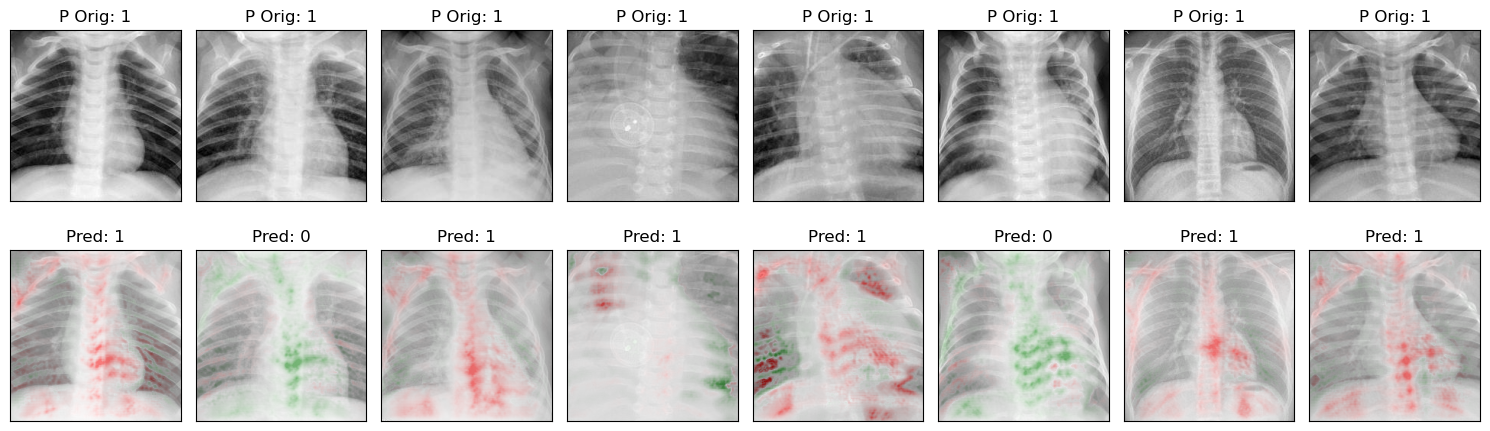
\includegraphics[width=1\textwidth]{images/ig_rand_test_P.png}
    \end{subfigure}
    \caption{Test images to which integrated gradients was applied. The model was finetuned on random labels. Upper two rows are from healthy patients, bottom two rows from patients with pneumonia. The 1st and 3rd row contain the input image, the 2nd and 4th row contain an added overlay from integrated gradients. In red is the negative attribution, in green the positive attribution.}
    \label{fig:ig_rand_test}
\end{figure}

Another interesting feature is how much focus the model puts on the diaphragm, which is more opaque when compared to lung tissue.

There does not seem to be a clear difference between features of patients labeled as healthy or sick (and the model predicts most patients as sick anyway).

In conclusion, it seems that the model fine-tuned on random labels simply looks at brighter areas, i.e. dense tissues such as bone. This shows that our initial 'true' model did in fact learn to correctly attribute certain areas of the X-ray to certain classes.

The same trends can be seen for the test data in Figure \ref{fig:ig_rand_test}.


\subsection*{B. Grad-CAM}

Note that instead of clipping the overlay at 0, like in Q4 (normal ReLU), we clip the values of the localization map at -0.5. The reason for this being that clipping at 0 simply gave a purple screen (0 values everywhere), due to the lack of attribution obtained from the model. In the paper, the authors mention that without ReLU, the localization maps sometimes highlight more than just the desired class and perform worse at localization. Still, since we only have two classes and would like to properly explain at least something, we opt to clip at -0.5.

In Figure \ref{fig:gc_rand_train}, observations are consistent with each other and between both classes. We can see an outline of the two lungs and the empty space surrounding the patients in all images in purple/blue/azure, showing that the model was mainly focusing on darker intensities (since we only look at negative values), agreeing with the green/yellow color.

\begin{figure*}
    \centering
    \begin{subfigure}{\textwidth}
        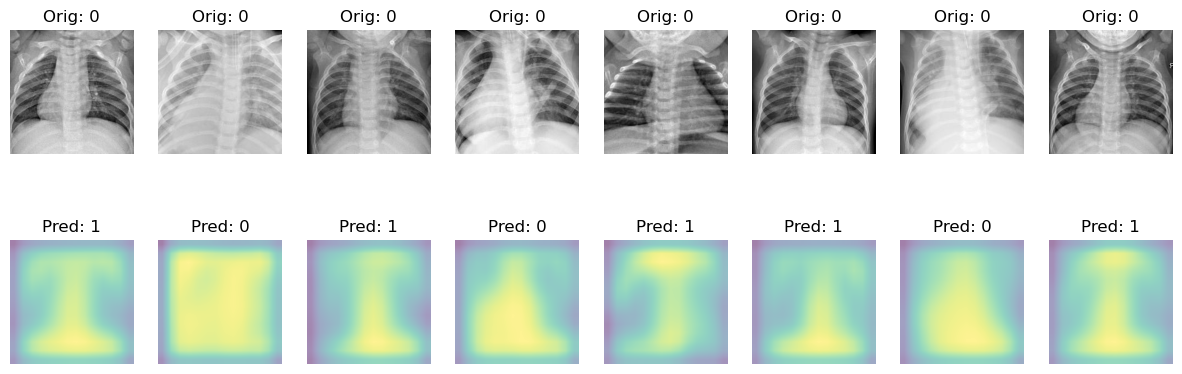
\includegraphics[width=1\textwidth]{images/gc_rand_train.png}
    \end{subfigure}
    \centering
    \begin{subfigure}{\textwidth}
        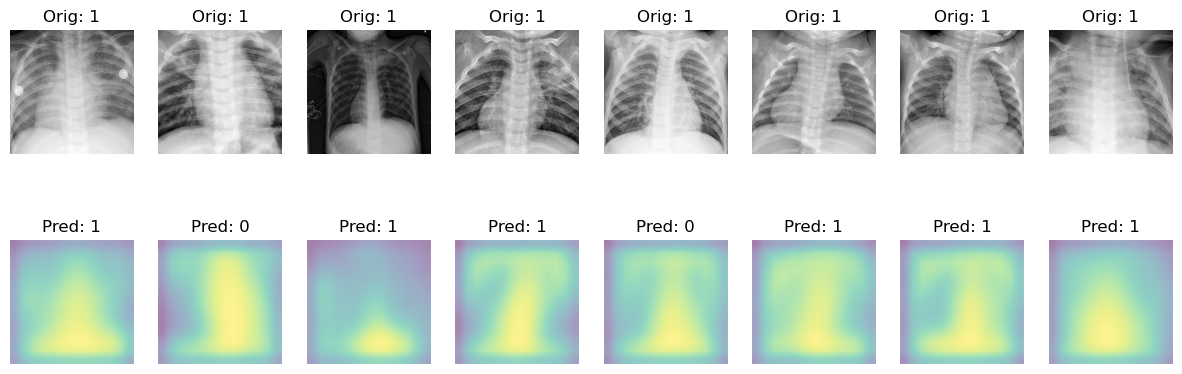
\includegraphics[width=1\textwidth]{images/gc_rand_train_P.png}
    \end{subfigure}
    \caption{Training images to which Grad-CAM was applied. The model was finetuned on random labels. Upper two rows are from healthy patients, bottom two rows from patients with pneumonia. The 1st and 3rd row contain the input image, the 2nd and 4th row contain the overlay produced by Grad-CAM. Yellow signifies the highest attribution, purple the lowest attribution.}
    \label{fig:gc_rand_train}
\end{figure*}

\begin{figure}
    \centering
    \begin{subfigure}{\columnwidth}
        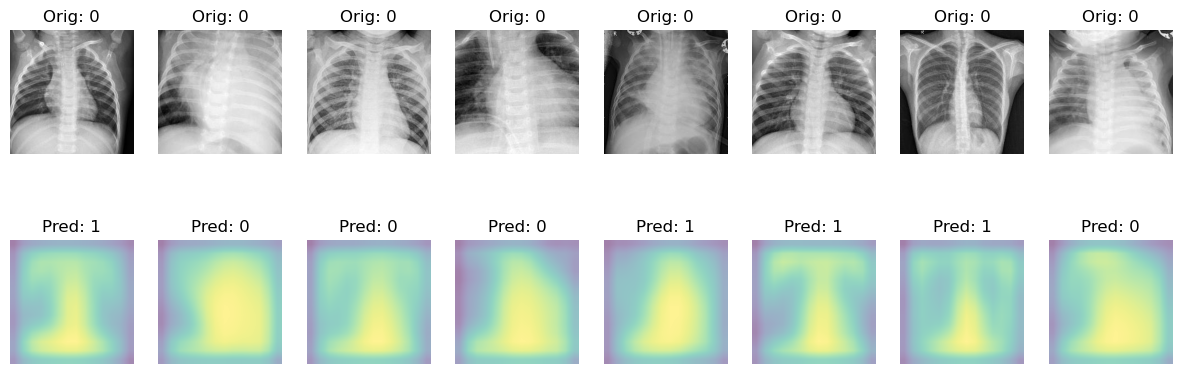
\includegraphics[width=1\textwidth]{images/gc_rand_test.png}
    \end{subfigure}
    \centering
    \begin{subfigure}{\columnwidth}
        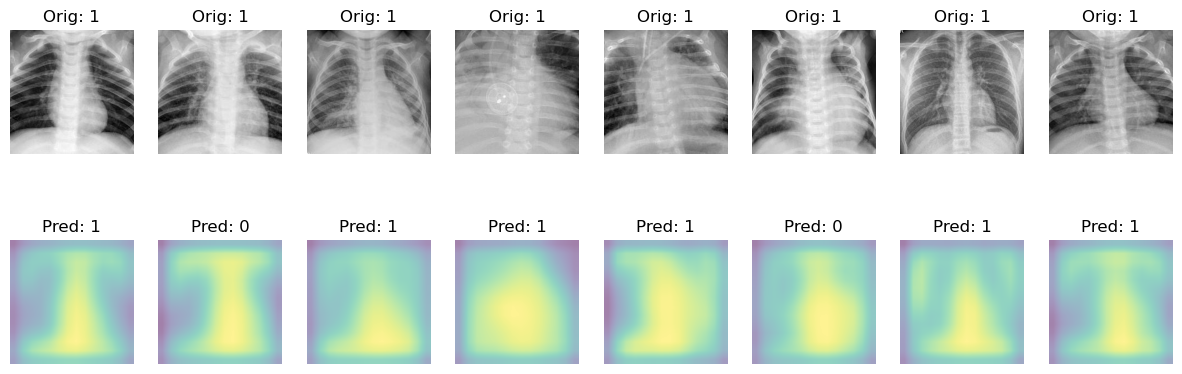
\includegraphics[width=1\textwidth]{images/gc_rand_test_P.png}
    \end{subfigure}
    \caption{Test images to which Grad-CAM was applied. The model was finetuned on random labels. Upper two rows are from healthy patients, bottom two rows from patients with pneumonia. The 1st and 3rd row contain the input image, the 2nd and 4th row contain the overlay produced by Grad-CAM. Yellow signifies the highest attribution, purple the lowest attribution.}
    \label{fig:gc_rand_test}
\end{figure}


Visualization of the test set in Figure \ref{fig:gc_rand_test} confirms the previously mentioned observations.
\section*{Challenge 2: Prototype Learning}
For challenge 2, we trained a kNN-classifier twice: once on random prototypes, and once on prototypes selected by the greedy algorithm.
To allow for easy computation of nearest neighbours, we flatten the images to a 1D array.

We train our first kNN-classifier (k=1) on a random subset of the training set and apply it to the validation set to calculate our metrics of interest (accuracy, precision, recall, and f1 score). More specifically, we do this for multiple values of S, with S the number of prototypes or the size of the subset.

We then move over to the greedy algorithm as mentioned in \cite{kim2016MMD}. For this we adapt the original code from the authors, which can be found at https://github.com/BeenKim/MMD-critic/blob/master/mmd.py. Since the paper mentioned that global kernels outperformed local ones, we opt to use only those.

\subsection*{A. Results}

When we train a kNN (k=1) classifier on random vs. greedy-selected prototypes, we get similar results in terms of accuracy, precision, and f1 score on the validation set, as shown in Figure \ref{fig:proto_metrics}. This shows that finding representative prototypes does not significantly help the classifier classify the samples more correctly. However, since recall is higher in most cases, training with greedy selection does seem to help reduce false negatives, which is useful when predicting serious diseases.

\begin{figure*}
    \centering
    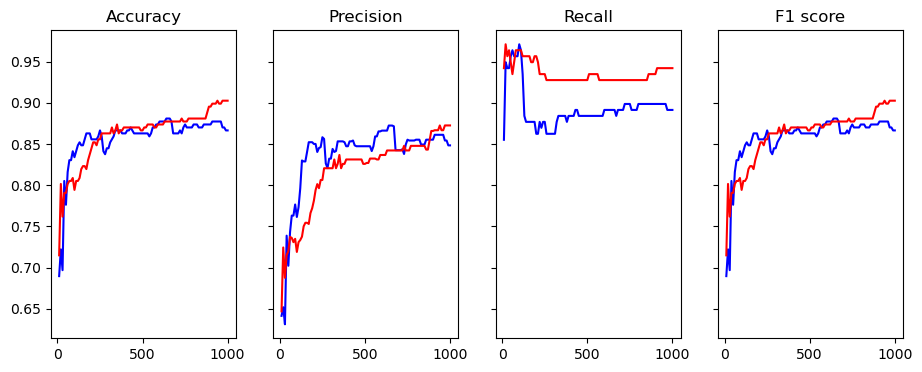
\includegraphics[width=0.8\textwidth]{images/proto_val_metrics.png}
    \caption{Accuracy, precision, recall, and f1 score on validation set. The blue plot shows the metrics for random prototype selection, the red plot for selection of prototypes with the greedy algorithm.}
    \label{fig:proto_metrics}
\end{figure*}


To obtain the final metrics on the test set, we choose the best classifier based on both the biggest difference in validation set accuracy and a minimum threshold for the accuracy of the greedy algorithm.
The accuracy of the model when using the greedy algorithm to select $S=990$ prototypes is slightly lower than random selection (79\% vs. 77\%), although this result varies depending on the initially selected random prototypes.

\begin{figure*}
    \centering
    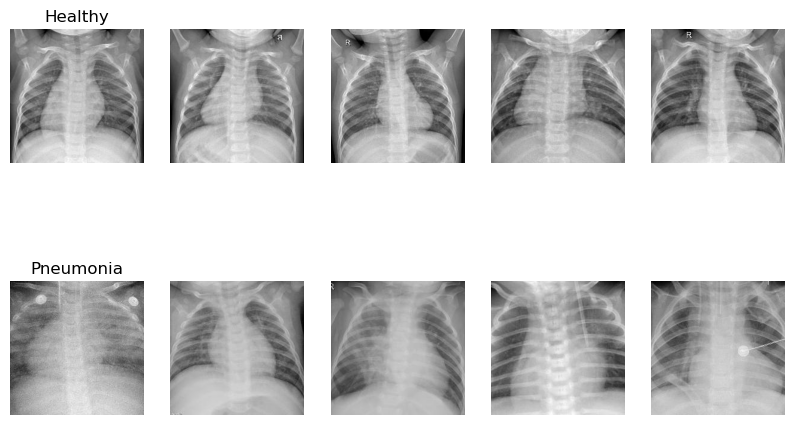
\includegraphics[width=0.8\textwidth]{images/prototypes.png}
    \caption{Prototypes of healthy (upper row) and sick (bottom row) patients, all selected by the greedy algorithm.}
    \label{fig:prototypes}
\end{figure*}

\subsection*{B. Prototype Inspection and Further Improvements}

Images from healthy patients seem relatively consistent with one another, while images from sick children vary widely (see Figure \ref{fig:prototypes}). For example, some images show clearly obfuscated lungs, while others seem to have similarly 'open' lungs, but instead thickening of the airways as the main radiological finding.

We could improve the general performance by finding criticisms, which can point to potential outliers or even mistakes in the dataset.
We could also use the output of integrated gradients, find prototypes and criticisms, and apply kNN to it.

When we compare this type of interpretable method to the previously seen saliency maps, in terms of visualization, the saliency maps provide much more information than the prototypes, simply because we see the contribution of certain features.
Of course, we can easily apply these saliency maps to the prototypes to get additional understanding on why these images might be considered good representatives of a certain class.
\section*{General Questions}

\subsection*{Q1: How consistent were the different interpretable/ explainable methods? Did they find similar patterns?}
Both integrated gradients (IG) and Grad-CAM were consistent for healthy patients (Grad-CAM more so than IG), but relatively inconsistent for sick patients (IG more so than Grad-CAM). Overall, integrated gradients was able to find more detailed patterns, while Grad-CAM seemed to focus mainly on the area of the lungs (which makes sense, since Grad-CAM is supposed to be a coarse-grained map). Interestingly, an overlapping pattern for both methods was the focus on the shoulder joint.

\subsection*{Q2: Given the “interpretable” or “explainable” results of one of the models, how would you explain and present them to a broad audience? Pick one example per part of the project.}
First we can discuss the medical background of the task: in part 2 this would be distinguishing patients with pneumonia from normal patients with the help of X-rays. We can talk about which radiological findings indicate pneumonia, and what features in general are important to look at (e.g. bone doesn't give any information, but lung tissue does).
Then, we can apply integrated gradients and look for images that most clearly highlight these areas we're interested in. We can also show some edge cases where the model seems to focus on an odd area (possibly due to a bias).


\subsection*{Q3: Did you encounter a tradeoff between accuracy and interpretability/explainability?}
When trained for 21 epochs, the model had a better accuracy than when trained for only 7 epochs, but when applying IG or Grad-CAM, the model ended up focusing on very specific, hard-to-attribute-to-disease features, that were seemingly patient-specific. An increase in accuracy therefore seems to be paired with a decrease in interpretability (although this might not necessarily be a linear relationship).

\subsection*{Q4: Do your findings from the interpretability/ explainability methods align with the current medical knowledge about these diseases?}
As mentioned in part 2 of the report, most tell-tale signs of pneumonia, such as thickening of the bronchi, opacification of the lung tissue, etc. were highlighted by IG. Grad-CAM only highlighted the lungs, which are of course the main area to be affected by pneumonia.

\subsection*{Q5: If you had to deploy one of the methods in practice, which one would you choose and why?}
For part 2, IG seems to be more interesting to look at, because of its ability to localize more fine-grained attributions. Still, if the observer does not possess enough medical knowledge, then Grad-CAM might be a better solution, due to its more coarse overlay and its ability to show the more general attribution.


%\printbibliography
\printbibliography[heading=references]

\end{document}
